\section{Teoria dellla computabilità}

\subsection{Fondamenti della Calcolabilità}
\subsubsection{Enumerabilità, computabilità e decidibilità}

\textbf{Cos'è un algoritmo?}
È una \textsc{nozione primitiva} $\longrightarrow$ non ha una definizione formale, ma lo abbiamo nella nostra testa e sappiamo riconoscerlo.

\vspace{0.4cm}
\textbf{Definizioni formali} \\
Per prima cosa ci mettiamo in un \underline{contesto formale}:
\begin{itemize}
    \item $\Sigma$ : alfabeto
    \item $\Sigma^*$ : stringhe finite su $\Sigma$
    \item $\mathcal{L} \subseteq \Sigma^*$ : linguaggio
\end{itemize}

\vspace{0.4cm}
\textbf{Definizione:} $\mathcal{L} \subseteq \Sigma^*$ si dice \textbf{DECIDIBILE} quando $\exists\ \mathcal{M}$ algoritmo che, data $w \in \Sigma^*$, mi dice in tempo finito se $w \in \mathcal{L}$ oppure $w \notin \mathcal{L}$.

\vspace{0.4cm}
\textbf{Definizione:} $\mathcal{L} \subseteq \Sigma^*$ si dice \textbf{ENUMERABILE} quando $\exists\ \mathcal{M}$ algoritmo che, fatto partire su input vuoto, \underline{produce la lista delle stringhe di $\mathcal{L}$} (ciascuna stringa in tempo finito).

\vspace{0.4cm}
\textbf{Definizione:} Siano $\Sigma_1, \Sigma_2$ alfabeti, $\mathcal{L}_1 \subseteq \Sigma_1^*$, $\mathcal{L}_2 \subseteq \Sigma_2^*$. \\
$f: \mathcal{L}_1 \to \mathcal{L}_2$ si dice \textbf{COMPUTABILE} quando $\exists\ \mathcal{M}$ algoritmo che, fatto partire su input $w \in \mathcal{L}_1$, restituisce $f(w) \in \mathcal{L}_2$ in tempo finito.

\vspace{0.4cm}
\textbf{Proposizione:} Sia $\Sigma$ un alfabeto.
$$\mathcal{L} \text{ DECIDIBILE} \implies \mathcal{L} \text{ ENUMERABILE}$$

\textit{Dimostrazione:} \\
Sia $\mathcal{M}$ un algoritmo di decisione per $\mathcal{L}$. Descrivo un algoritmo di enumerazione per $\mathcal{L}$:
$\forall\ $ stringa $w \in \Sigma^*$, eseguo $\mathcal{M}$ su $w$:
\begin{itemize}
    \item Se $w \in \mathcal{L}$, aggiungo $w$ alla lista.
    \item Se $w \notin \mathcal{L}$, non l'aggiungo.
\end{itemize}

\vspace{0.4cm}
\textbf{Osservazione:} $\Sigma$ numerabile $\implies \Sigma^*$ enumerabile. \\
Sia $\Sigma = \{a_1, a_2, \dots, a_n, \dots\}$. \\
Se cerchiamo di enumerare le stringhe di lunghezza 2 su $\Sigma$ tramite un \textsc{Procedimento Diagonale di Cantor}:

$$\renewcommand{\arraystretch}{1.2}
\begin{array}{c|ccccccc}
 & a_1 & & a_2 & & a_3 & & \dots \\
\hline
a_1 & a_1 a_1 & \rightarrow & a_1 a_2 & & a_1 a_3 & \rightarrow & \dots \\
 & & \swarrow & & \nearrow & & \swarrow & \\
a_2 & a_2 a_1 & & a_2 a_2 & & a_2 a_3 & & \dots \\
 & \downarrow & \nearrow & & \swarrow & & & \\
a_3 & a_3 a_1 & & a_3 a_2 & & \dots & & \\
 & & \swarrow & & & & & \\
\vdots & \vdots & & \vdots & & & & \ddots
\end{array}$$


Usando il procedimento diagonale è possibile enumerare le parole e poi trovare un algoritmo di enumerazione per le stringhe.

\vspace{0.4cm}
\textbf{Attenzione:} $\mathcal{L} \text{ decidibile} \impliedby \mathcal{L} \text{ enumerabile}$ (NON vale il viceversa in generale). \\
MA vale la seguente...

\vspace{0.4cm}
\textbf{Proposizione:} 
$$\mathcal{L} \text{ DECIDIBILE} \iff \mathcal{L} \text{ ENUMERABILE e } \mathcal{L}^c \text{ ENUMERABILE} \quad (\text{dove } \mathcal{L}^c = \Sigma^* \setminus \mathcal{L})$$

\textit{Dimostrazione:}
\begin{itemize}
    \item[$\implies$)] $\mathcal{L}$ decidibile $\implies \mathcal{L}$ enumerabile (già dimostrato, OK). \\
    $\mathcal{L}$ decidibile $\implies \mathcal{L}^c$ enumerabile: analogo.
    
    \item[$\impliedby$)] Sia $\mathcal{M}$ algoritmo di enumerazione per $\mathcal{L}$: $w_1, w_2, w_3, \dots, w_n, \dots$ \\
    Sia $\mathcal{M}^c$ algoritmo di enumerazione per $\mathcal{L}^c$: $v_1, v_2, v_3, \dots, v_n, \dots$ \\
    Costruisco un algoritmo di decisione per $\mathcal{L}$: \\
    Su input $w \in \Sigma^*$, eseguo $\mathcal{M}$ e $\mathcal{M}^c$ in maniera \textsc{alternata}.
    Ogni volta che viene prodotta una stringa $X$, la confronto con $w$:
    \begin{itemize}
        \item Se $X \neq w$, proseguo.
        \item Se $X = w$ e $X$ è prodotta da $\mathcal{M}$, accetto $w$.
        \item Se $X = w$ e $X$ è prodotta da $\mathcal{M}^c$, rifiuto $w$.
    \end{itemize}
\end{itemize}

\vspace{0.4cm}
\textbf{Definizione:} $\mathcal{L} \subseteq \Sigma^*$ si dice \textbf{SEMIDECIDIBILE} quando $\exists\ \mathcal{M}$ algoritmo che, fatto partire su input $w$:
\begin{itemize}
    \item Se $w \in \mathcal{L}$, termina e accetta $w$.
    \item Se $w \notin \mathcal{L}$, può non terminare (va in loop).
\end{itemize}

\vspace{0.4cm}
\textbf{Osservazione:} $\mathcal{L}$ semidecidibile $\iff \exists\ \mathcal{M}$ algoritmo che, su input $w$:
\begin{itemize}
    \item Se $w \in \mathcal{L}$, termina e accetta $w$.
    \item Se $w \notin \mathcal{L}$, non termina.
\end{itemize}

\vspace{0.4cm}
\textbf{Proposizione:}
$$\mathcal{L} \text{ ENUMERABILE} \iff \mathcal{L} \text{ SEMIDECIDIBILE}$$

\textit{Dimostrazione:}
\begin{itemize}
    \item[$\implies$)] Sia $\mathcal{M}$ algoritmo di enumerazione per $\mathcal{L}$: $w_1, w_2, w_3, \dots$ \\
    Costruisco un algoritmo di semidecisione per $\mathcal{L}$: \\
    Data $w \in \Sigma^*$, confronto $w$ con le stringhe prodotte via via da $\mathcal{M}$. Se $w$ è tra queste, termino e accetto $w$.
    
    \item[$\impliedby$)] Sia $\mathcal{M}$ algoritmo di semidecisione per $\mathcal{L}$ (che non termina su tutte le stringhe del complemento). \\
    Eseguo i passi di computazione intrecciandoli (dovetailing):
    $$
    \renewcommand{\arraystretch}{1.2}
    \begin{array}{l|ccccccc}
    w_1: & x & & x & & x & \dots & x \\
         & & \swarrow & & \nearrow & & \swarrow & \\
    w_2: & x & & x & & x & \dots & \circ \\
         & \downarrow & \nearrow & & \swarrow & & & \\
    w_3: & x & & x & & \dots & & \\
         & & \swarrow & & & & & \\
    w_4: & x & & \dots & & & & \\
    \vdots & \vdots & & & & & &
    \end{array}
    $$
    \textit{(Eseguo 1 passo su $w_1$; poi 1 passo su $w_1$ e 1 su $w_2$; poi 1 passo su $w_1$, $w_2$ e $w_3$, ecc. Quando una computazione termina e accetta (es. in $w_2$), metto la stringa corrispondente nella lista).}\end{itemize}

\vspace{0.4cm}
\textbf{Definizione:} $\mathcal{L} \subseteq \Sigma^*$ si dice avere \textbf{FUNZIONE CARATTERISTICA} $\chi_\mathcal{L}$ se la funzione è così definita:
$$ 
\chi_\mathcal{L} : \Sigma^* \to \{0, 1\} \quad : \quad w \mapsto 
\begin{cases} 
0, & w \notin \mathcal{L} \\ 
1, & w \in \mathcal{L} 
\end{cases}
$$

\vspace{0.4cm}
\textbf{Proposizione:}
$$\mathcal{L} \text{ DECIDIBILE} \iff \chi_\mathcal{L} \text{ COMPUTABILE}$$

\textit{Dimostrazione:}
\begin{itemize}
    \item[$\implies$)] Sia $\mathcal{M}$ algoritmo di decisione per $\mathcal{L}$. Costruisco un algoritmo di calcolo per $\chi_\mathcal{L}$: \\
    Data $w \in \Sigma^*$, eseguo $\mathcal{M}$ su $w$:
    \begin{itemize}
        \item Se $w \in \mathcal{L}$, scrivo 1.
        \item Se $w \notin \mathcal{L}$, scrivo 0.
    \end{itemize}
    \item[$\impliedby$)] Sia $\mathcal{M}$ algoritmo di calcolo per $\chi_\mathcal{L}$. Costruisco un algoritmo di decisione per $\mathcal{L}$: \\
    Su input $w$, calcolo $\chi_\mathcal{L}(w)$ (usando $\mathcal{M}$):
    \begin{itemize}
        \item Se $\chi_\mathcal{L}(w) = 1$, $w \in \mathcal{L}$.
        \item Se $\chi_\mathcal{L}(w) = 0$, $w \notin \mathcal{L}$.
    \end{itemize}
\end{itemize}

\vspace{0.4cm}
\textbf{Proposizione:} Siano $\mathcal{L}_1, \mathcal{L}_2 \subseteq \Sigma^*$ DECIDIBILI. Allora:
\begin{enumerate}
    \item $\mathcal{L}_1 \cup \mathcal{L}_2$ è decidibile
    \item $\mathcal{L}_1 \cap \mathcal{L}_2$ è decidibile
    \item $\mathcal{L}_1^c$ è decidibile
\end{enumerate}

\textit{Dimostrazione:}
\begin{enumerate}
    \item \textbf{Algoritmo di decisione per $\mathcal{L}_1 \cup \mathcal{L}_2$}: \\
    Su input $w$: Eseguo $\mathcal{M}_1$. Se $w \in \mathcal{L}_1$ termino e accetto. \\
    Se $w \notin \mathcal{L}_1$, eseguo $\mathcal{M}_2$:
    \begin{itemize}
        \item Se $w \in \mathcal{L}_2$, termino e accetto.
        \item Altrimenti rifiuto.
    \end{itemize}
    
    \item \textbf{Algoritmo di decisione per $\mathcal{L}_1 \cap \mathcal{L}_2$}: \\
    Su input $w$: Eseguo $\mathcal{M}_1$:
    \begin{itemize}
        \item Se $w \notin \mathcal{L}_1$, rifiuto.
        \item Se $w \in \mathcal{L}_1$, osservo $\mathcal{M}_2$:
        \begin{itemize}
            \item Se $w \notin \mathcal{L}_2$, rifiuto.
            \item Altrimenti accetto.
        \end{itemize}
    \end{itemize}
    
    \item \textbf{Algoritmo di decisione per $\mathcal{L}_1^c$}: \\
    Su input $w$, eseguo $\mathcal{M}_1$ e \textsc{scambio le sue risposte} (cioè l'algoritmo di decisione inverte l'output).
\end{enumerate}

\vspace{0.6cm}
% --- NUOVA SOTTOSEZIONE: FUNZIONI RICORSIVE ---
\subsection{Funzioni Ricorsive}
\subsubsection{Funzioni ricorsive primitive}

Ci concentriamo su funzioni del tipo:
$$f: \mathbb{N}^k \to \mathbb{N}$$
$$(x_1, \dots, x_k) \in \mathbb{N}^k$$
$$f(x_1, \dots, x_k)$$
Indicheremo il vettore di input come $\vec{x} = (x_1, \dots, x_k)$.

\vspace{0.4cm}
\textbf{FUNZIONI INIZIALI}
\begin{enumerate}
    \item \textbf{Costanti k-arie di valore 0}:
    $$C_0^{(k)} : \mathbb{N}^k \to \mathbb{N}$$
    $$C_0^{(k)}(\vec{x}) = 0$$
    
    \item \textbf{Funzione successore}:
    $$S : \mathbb{N} \to \mathbb{N}$$
    $$S(x) = x + 1$$
    
    \item \textbf{Proiezioni j-esime k-arie}:
    $$\mathcal{E}_j^{(k)} : \mathbb{N}^k \to \mathbb{N}$$
    $$\mathcal{E}_j^{(k)}(\vec{x}) = x_j \quad \text{(estrae l'argomento j-esimo)}$$
\end{enumerate}

\vspace{0.4cm}
\textbf{Definizione:} Sia $A$ un insieme, $\Sigma$ un alfabeto. \\
Una \textbf{Codifica} è una funzione $p: A \to \Sigma^*$ (da $A$ ottengo una stringa).

\vspace{0.4cm}
\textbf{Definizione:} Una \textbf{Rappresentazione} (Buona codifica) di $A$ in $\Sigma$ si ha quando:
\begin{enumerate}
    \item $p$ è \textbf{computabile} ($\exists\ $ algoritmo che per $\forall\ a \in A$ mi calcola $p(a)$).
    \item $p$ è \textbf{iniettiva} (la codifica è unica).
    \item $p(A)$ è \textbf{decidibile} e $p$ è \textbf{effettivamente invertibile}, cioè: $\exists\ $ un algoritmo che, $\forall\ w \in p(A)$, mi restituisce $a \in A$ tale che $p(a) = w$ (Posso ricostruire senza ambiguità l'elemento di $A$ dalla codifica).
\end{enumerate}

\vspace{0.4cm}
\textbf{Proposizione:} Sia $\Sigma$ un alfabeto. Allora $\exists\ p$ rappresentazione in $\{0, 1\}^*$. \\
$p : \Sigma^* \to \{0, 1\}^*$ (Posso codificare in binario).

\textit{Dimostrazione:} \\
Sia $\Sigma = \{a_1, a_2, \dots, a_n, \dots\}$. \\
$p : \Sigma^* \to \{0, 1\}^*$ \\
$p(a_{i_1} a_{i_2} \dots a_{i_n}) = 01\dots101\dots1\dots01\dots1$ (dove i blocchi di $1$ dipendono dagli indici $i_k$). \\
$p$ è una rappresentazione di $\Sigma^*$ in $\{0, 1\}^*$.

\vspace{0.4cm}
\textbf{Codifica unaria per numeri naturali:} \\
$\Sigma = \{1\}$ \\
$0 \mapsto 1$ \\
$1 \mapsto 11$ \\
$2 \mapsto 111$ \\
$n \mapsto \underbrace{11\dots1}_{n+1 \text{ volte}}$

\vspace{0.4cm}
\textbf{Osservazione:} Le funzioni iniziali sono computabili. \\
Esempio: $S(\underbrace{11\dots1}_{n+1}) = \underbrace{1\dots1}_{n+2}$

\vspace{0.4cm}
\textbf{Definizione: Composizione generalizzata} \\
Date $g_1 \dots g_n : \mathbb{N}^k \to \mathbb{N}$ e $f : \mathbb{N}^n \to \mathbb{N}$. \\
La \textbf{composizione generalizzata} (o sostituzione) di $f$ con $(g_1, \dots, g_n)$ è la funzione:
$$f \circ (g_1, \dots, g_n) : \mathbb{N}^k \to \mathbb{N}$$
$$(f \circ (g_1, \dots, g_n))(\vec{x}) = f(g_1(\vec{x}), \dots, g_n(\vec{x}))$$

\vspace{0.4cm}
\textbf{Proposizione:} $f, g_1, \dots, g_n$ computabili $\implies f \circ (g_1, \dots, g_n)$ computabile.

\textit{Dimostrazione:} \\
Siano $F, G_1, \dots, G_n$ algoritmo di calcolo per $f, g_1, \dots, g_n$. \\
Algoritmo di calcolo per $f \circ (g_1, \dots, g_n)$: \\
Data $\vec{x} \in \mathbb{N}^k$:
\begin{itemize}
    \item Uso $G_1, \dots, G_n$ per calcolare $g_1(\vec{x}), \dots, g_n(\vec{x})$.
    \item Uso $F$ per calcolare $f(g_1(\vec{x}), \dots, g_n(\vec{x}))$.
\end{itemize}

\vspace{0.4cm}
\textbf{Definizione: Ricorsione Primitiva (RP)} \\
Date $g: \mathbb{N}^k \to \mathbb{N}$, $\varphi : \mathbb{N}^{k+2} \to \mathbb{N}$. \\
Diciamo che $f: \mathbb{N}^{k+1} \to \mathbb{N}$ è definita per \textbf{ricorsione primitiva} (RP) da $g$ e $\varphi$ quando:
\begin{itemize}
    \item $f(\vec{x}, 0) = g(\vec{x})$  \textit{(caso base)}
    \item $f(\vec{x}, y+1) = \varphi(\vec{x}, y, f(\vec{x}, y))$ \textit{(passo induttivo)}
\end{itemize}

\vspace{0.4cm}
\textbf{Proposizione:} $g, \varphi$ computabili $\implies f$ definita per RP da $g, \varphi$ è computabile.

\textit{Dimostrazione:} \\
Descrivo un algoritmo per calcolare $f$, ragionando per induzione sull'ultimo parametro di $f$. In pratica facciamo vedere che fissato $\vec{x} \in \mathbb{N}^k$, per ogni $y \in \mathbb{N}$, so calcolare $f(\vec{x}, y)$:
\begin{itemize}
    \item (Base $y=0$): $f(\vec{x}, 0) = g(\vec{x})$, e $g$ è computabile.
    \item (Iterazione): Supponiamo di saper calcolare $f(\vec{x}, y)$. \\
    $f(\vec{x}, y+1) = \varphi(\vec{x}, y, f(\vec{x}, y))$. Essendo $\varphi$ computabile (per hp) e $f(\vec{x},y)$ noto, anche il calcolo al passo successivo restituisce un risultato in tempo finito.
\end{itemize}

\vspace{0.4cm}
\textbf{Definizione: Derivazione Ricorsiva Primitiva (drp)} \\
È una sequenza di funzioni $f_1, f_2, \dots, f_n$ t.c. $\forall\ i = 1, \dots, n$:
\begin{itemize}
    \item $f_i$ è \textbf{funzione iniziale}, oppure
    \item $f_i$ è \textbf{ottenuta da $f_j, f_k$ per RP} con $j, k < i$, oppure
    \item $f_i$ è \textbf{ottenuta per composizione generalizzata} da funzioni precedenti 
\end{itemize}

\vspace{0.4cm}
\textbf{Definizione: Funzione Ricorsiva Primitiva (rp)} \\
Una \textbf{funzione ricorsiva primitiva (rp)} è una funzione che compare in coda ad una drp (ovvero è l'ultima funzione di una drp).

\newpage
\textbf{Osservazione:}
\begin{enumerate}
    \item Ogni prefisso di una drp è una drp.
    \item Ogni funzione che compare in una drp è rp.
\end{enumerate}

\vspace{0.4cm}
\textbf{Proposizione:} \textbf{Ogni funzione rp è computabile.}

\textit{Dimostrazione:} \\
Sia $f$ rp. Dimostro per \textbf{induzione sulla lunghezza $n$ di una drp} che termina con $f$:
\begin{itemize}
    \item \textbf{Caso base ($n=1$)}: $f \implies f$ è funzione iniziale, dunque è computabile.
    \item \textbf{Passo induttivo}: Supponiamo che tutte le funzione che compaiono in una drp di lunghezza $< n$ siano computabili. \\
    Sia $f_1, \dots, f_n = f$. \\
    $f$ deriva da funzioni precedenti $f_j, \dots, f_k$ le quali sono computabili per Hp induttiva. Siccome le operazioni di composizione e RP mantengono la computabilità (come dimostrato in precedenza), anche $f$ è computabile.
\end{itemize}

\vspace{0.6cm}
\textbf{Proposizione:}
\begin{enumerate}
    \item $g: \mathbb{N}^k \to \mathbb{N}$, $\varphi: \mathbb{N}^{k+2} \to \mathbb{N}$ rp $\implies f$ ottenuta per RP da $g$ e $\varphi$ è rp.
    \item $\varphi: \mathbb{N}^n \to \mathbb{N}$, $g_1, \dots, g_n: \mathbb{N}^k \to \mathbb{N}$ rp $\implies f \circ (g_1, \dots, g_n)$ rp.
\end{enumerate}

\textit{Dimostrazione:}
\begin{enumerate}
    \item Siano $g_1, \dots, g_s, g$ una drp per $g$, e $\varphi_1, \dots, \varphi_r, \varphi$ una drp per $\varphi$. \\
    La sequenza $g_1, \dots, g_s, g, \varphi_1, \dots, \varphi_r, \varphi, f$ è essa stessa una drp (poiché per ipotesi tutte le precedenti sono drp e $f$ è ottenuta da esse). Di conseguenza, $f$ è rp perché compare in una drp.
\end{enumerate}

\vspace{0.6cm}
\textbf{ESEMPI DI FUNZIONI RICORSIVE PRIMITIVE}

\vspace{0.4cm}
\textbf{1) Costante m-esima k-aria:} $C_m^{(k)} : \mathbb{N}^k \to \mathbb{N}$, dove $C_m^{(k)}(x_1, \dots, x_k) = m \quad (m \in \mathbb{N})$, con k che indica il numero di argomenti (es. $C_0^{(2)}(x,y) = 0$) e m che indica il valore della costante (es. $C_3^{(2)}(x,y) = 3$).
Dimostriamo per induzione su $m \in \mathbb{N}$ che è rp:
\begin{itemize}
    \item Base: $C_0^{(k)}$ è rp (perché è una \textbf{funzione iniziale}).
    \item Supponiamo che $C_m^{(k)}$ sia rp. \\
    $C_{m+1}^{(k)}(\vec{x}) = m+1 = (S \circ C_m^{(k)})(\vec{x})$ \\
    Essendo la composizione tra $S$ (funzione successore, che è iniziale) e $C_m^{(k)}$ (rp per ipotesi induttiva), allora $C_{m+1}^{(k)}$ è rp.
\end{itemize}

\vspace{0.4cm}
\textbf{2) Funzione Predecessore:} $v : \mathbb{N} \to \mathbb{N}$
$$
v(x) = \begin{cases} 
x-1, & x > 0 \\ 
0, & x = 0 
\end{cases}
$$
Costruiamo la ricorsione primitiva:
$$
\begin{cases} 
v(0) = 0 \quad \text{(che corrisponde a $C_0^{(0)}$ che è rp)} \\ 
v(x+1) = \left( \mathcal{E}_1^{(2)} \right)(x, v(x)) = x \quad \text{(rp perché $\mathcal{E}_1^{(2)}$ è funz. iniziale)}
\end{cases}
$$
$\implies v(x)$ è rp.

\vspace{0.4cm}
\textbf{3) Somma:} $s : \mathbb{N}^2 \to \mathbb{N}$ \\
$s(x,y) = x+y$
$$
\begin{cases} 
s(x,0) = x = \mathcal{E}_1^{(1)}(x) \quad \text{(rp)} \\ 
s(x, y+1) = x+y+1 = \left( S \circ \mathcal{E}_3^{(3)} \right)(x, y, s(x,y)) \quad \text{(rp)}
\end{cases}
$$
$\implies s$ è rp.

\vspace{0.4cm}
\textbf{4) Prodotto:} $p : \mathbb{N}^2 \to \mathbb{N}$ \\
$p(x,y) = x \cdot y$
$$
\begin{cases} 
p(x,0) = 0 = \left( C_0^{(1)} \right)(x) \quad \text{(rp)} \\ 
p(x, y+1) = xy + x = \left( s \circ (\mathcal{E}_3^{(3)}, \mathcal{E}_1^{(3)}) \right)(x, y, p(x,y)) \quad \text{(rp)}
\end{cases}
$$
$\implies p$ è rp.

\vspace{0.4cm}
\textbf{5) Esponenziazione:} $\pi : \mathbb{N}^2 \to \mathbb{N}$ \\
$\pi(x,y) = x^y$
$$
\begin{cases} 
\pi(x,0) = x^0 = 1 = C_1^{(1)}(x) \quad \text{(rp)} \\ 
\pi(x, y+1) = x^y \cdot x = \left( p \circ (\mathcal{E}_3^{(3)}, \mathcal{E}_1^{(3)}) \right)(x, y, \pi(x,y)) \quad \text{(rp)}
\end{cases}
$$

\vspace{0.4cm}
\textbf{6) Fattoriale:} $f : \mathbb{N} \to \mathbb{N}$ \\
$f(x) = x!$
$$
\begin{cases} 
f(0) = 1 \quad \text{(rp)} \\ 
f(x+1) = (x+1)! = (x+1) \cdot x! = \left( p \circ (S \circ \mathcal{E}_1^{(2)}, \mathcal{E}_2^{(2)}) \right)(x, f(x))
\end{cases}
$$

\vspace{0.4cm}
\textbf{7) Differenza Troncata:} $\overset{\cdot}{-} : \mathbb{N}^2 \to \mathbb{N}$
$$
x \overset{\cdot}{-} y = \begin{cases} 
x-y, & x \ge y \\ 
0, & x < y 
\end{cases}
$$
$$
\begin{cases} 
x \overset{\cdot}{-} 0 = x = \mathcal{E}_1^{(1)}(x) \quad \text{(rp)} \\ 
x \overset{\cdot}{-} (y+1) = x-y-1 = \left( v \circ \mathcal{E}_3^{(3)} \right)(x, y, x \overset{\cdot}{-} y) \quad \text{(rp)}
\end{cases}
$$

\vspace{0.4cm}
\textbf{8) Distanza:} $d : \mathbb{N}^2 \to \mathbb{N}$ \\
$d(x,y) = |x-y|$
$$ d(x,y) = (x \overset{\cdot}{-} y) + (y \overset{\cdot}{-} x) $$
(Questo copre entrambi i casi in cui $x \ge y$ o $y > x$)
$$ = \left( s \circ (\overset{\cdot}{-} \circ (\mathcal{E}_1^{(2)}, \mathcal{E}_2^{(2)}), \overset{\cdot}{-} \circ (\mathcal{E}_2^{(2)}, \mathcal{E}_1^{(2)})) \right)(x,y) $$
$\implies d$ è rp.

\vspace{0.4cm}
\textbf{9) Segno:} $sg : \mathbb{N} \to \mathbb{N}$
$$
sg(x) = \begin{cases} 
1, & x > 0 \\ 
0, & x = 0 
\end{cases}
$$
$$
\begin{cases} 
sg(0) = 0 \\ 
sg(x+1) = 1 = C_1^{(2)}(x, sg(x)) 
\end{cases}
$$
\textbf{10) Segno Opposto:} $\overline{sg} : \mathbb{N} \to \mathbb{N}$
$$
\overline{sg}(x) = \begin{cases} 
0, & x > 0 \\ 
1, & x = 0 
\end{cases}
$$

\textit{Dimostrazione:}
Possiamo dimostrare che è rp per ricorsione primitiva:
$$
\begin{cases} 
\overline{sg}(0) = 1 = C_1^{(0)} \quad \text{(rp)} \\ 
\overline{sg}(x+1) = 0 = C_0^{(2)}(x, \overline{sg}(x)) \quad \text{(rp, con composizione di proiezioni se necessario)}
\end{cases}
$$
$\implies \overline{sg}$ è rp.

\textit{Metodo alternativo (per composizione):}
Possiamo sfruttare la differenza troncata. Sottrarre $x$ a $1$ ci restituisce $1$ solo se $x=0$, altrimenti ci restituisce $0$:
$$ \overline{sg}(x) = 1 \overset{\cdot}{-} x = \left( \overset{\cdot}{-} \circ (C_1^{(1)}, \mathcal{E}_1^{(1)}) \right)(x) $$
Essendo ottenuta per composizione di funzioni rp, è rp.

\vspace{0.4cm}
\textbf{11) Delta di Kronecker:} $\delta(x,y)$
$$
\delta(x,y) = \begin{cases} 
1, & x = y \\ 
0, & x \neq y 
\end{cases}
$$

\textit{Dimostrazione:}
Sappiamo che la funzione distanza $d(x,y) = |x-y|$ (che abbiamo già dimostrato essere rp) vale $0$ se e solo se $x = y$, ed è strettamente maggiore di $0$ altrimenti.
Se applichiamo la funzione \textit{Segno Opposto} al risultato della distanza, otteniamo esattamente il comportamento del Delta di Kronecker:
$$ \delta(x,y) = \overline{sg}(d(x,y)) = \left( \overline{sg} \circ d \right)(x,y) $$
Essendo il Delta di Kronecker ottenuto per composizione di due funzioni rp ($\overline{sg}$ e $d$), è esso stesso una funzione rp.

\vspace{0.6cm}
\textbf{Definizione: Operatore di Somma Limitata} \\
Sia $f : \mathbb{N}^{k+1} \to \mathbb{N}$. Definiamo $g : \mathbb{N}^{k+1} \to \mathbb{N}$ ponendo:
$$ g(\vec{x}, z) = \sum_{y=0}^{z} f(\vec{x}, y) $$
Diciamo che $g$ è ottenuta per \textbf{somma limitata} da $f$. La funzione che, data $f$, costruisce $g$ si chiama operatore di somma limitata.

\vspace{0.4cm}
\textbf{Proposizione:} $f$ rp $\implies g$ ottenuta per somma limitata da $f$ è rp.

\textit{Dimostrazione:}
$$
\begin{cases} 
g(\vec{x}, 0) = \sum_{y=0}^{0} f(\vec{x}, y) = f(\vec{x}, 0) = \left( f \circ (\mathcal{E}_1^{(k)}, \mathcal{E}_2^{(k)}, \dots, \mathcal{E}_k^{(k)}, C_0^{(k)}) \right)(\vec{x}) \\ 
\\
g(\vec{x}, z+1) = \sum_{y=0}^{z+1} f(\vec{x}, y) = \sum_{y=0}^{z} f(\vec{x}, y) + f(\vec{x}, z+1) = \\
= \left( s \circ (\mathcal{E}_{k+2}^{(k+2)}, f \circ (\mathcal{E}_1^{(k+2)}, \dots, \mathcal{E}_k^{(k+2)}, S \circ \mathcal{E}_{k+1}^{(k+2)})) \right)(\vec{x}, z, g(\vec{x}, z)) 
\end{cases}
$$

\vspace{0.4cm}
\textbf{Osservazione:} \\
Data $f: \mathbb{N}^{k+2} \to \mathbb{N}$, possiamo avere $g: \mathbb{N}^{k+1} \to \mathbb{N}$ definita come:
$$ g(\vec{x}, z) = \sum_{y=0}^{z} f(\vec{x}, y, z) $$

\vspace{0.4cm}
\textbf{Definizione: Operatore di Prodotto Limitato} \\
Sia $f : \mathbb{N}^{k+1} \to \mathbb{N}$. Definiamo $g : \mathbb{N}^{k+1} \to \mathbb{N}$ ponendo:
$$ g(\vec{x}, z) = \prod_{y=0}^{z} f(\vec{x}, y) $$
Diciamo che $g$ è ottenuta per \textbf{prodotto limitato} da $f$.

\vspace{0.4cm}
\textbf{Proposizione:} $f$ rp $\implies g$ rp. \\
\textit{(La dimostrazione è la stessa della somma limitata, sostituendo l'operatore di somma $s$ con quello di prodotto $p$)}.

\vspace{0.6cm}
\textbf{Esercizio} \\
Sia $g: \mathbb{N}^2 \to \mathbb{N}$ una funzione rp.
\begin{enumerate}
    \item[a)] Sia $f_1(x, y, z_1, \dots, z_n) = g(x, y)$. Dimostrare che $f_1$ è rp:
    $$ f_1(x, y, z_1, \dots, z_n) = g(x, y) = \left( g \circ (\mathcal{E}_1^{(n+2)}, \mathcal{E}_2^{(n+2)}) \right)(x, y, z_1, \dots, z_n) $$
    
    \item[b)] Sia $f_2(x, y) = g(y, x)$. Dimostrare che $f_2$ sia rp:
    $$ f_2(x, y) = \left( g \circ (\mathcal{E}_2^{(2)}, \mathcal{E}_1^{(2)}) \right)(x, y) $$
    
    \item[c)] Sia $f_3(x) = g(x, x)$. Dimostrare che $f_3$ sia rp:
    $$ f_3(x) = \left( g \circ (\mathcal{E}_1^{(1)}, \mathcal{E}_1^{(1)}) \right)(x) $$
\end{enumerate}



%02/03/2026

\vspace{0.6cm}
\subsubsection{Relazioni ricorsive primitive}

\textbf{Definizione:} Sia $R \subseteq \mathbb{N}^k$. Una funzione $f: \mathbb{N}^k \to \mathbb{N}$ si dice \textbf{BUONA per $R$} quando:
$$ \forall\ \vec{x} \in \mathbb{N}^k, \quad f(\vec{x}) = 0 \iff \vec{x} \in R $$

\vspace{0.4cm}
\textbf{Definizione:} $R \subseteq \mathbb{N}^k$ (relazione k-aria) si dice \textbf{RICORSIVA PRIMITIVA (rp)} quando:
$$ \exists\ f: \mathbb{N}^k \to \mathbb{N} \text{ rp t.c. } \forall\ \vec{x} \in \mathbb{N}^k, \quad f(\vec{x}) = 0 \iff \vec{x} \in R $$
(cioè esiste $f$ rp che è buona per $R$).

\vspace{0.4cm}
\textbf{Osservazione:} $R \subseteq \mathbb{N}^k$ è rp $\iff \chi_R$ (FUNZIONE CARATTERISTICA di $R$) è rp.
$$
\chi_R : \mathbb{N}^k \to \mathbb{N}, \quad \chi_R(\vec{x}) = 
\begin{cases} 
1, & \text{se } \vec{x} \in R \\ 
0, & \text{se } \vec{x} \notin R 
\end{cases}
$$

\textit{Dimostrazione:}
\begin{itemize}
    \item[$\implies$)] $R$ rp $\implies$ sia $f: \mathbb{N}^k \to \mathbb{N}$ rp BUONA PER $R$.
    $$ \chi_R(\vec{x}) = (\overline{sg} \circ f)(\vec{x}) $$
    Essendo $\overline{sg}$ rp e $f$ rp (per ipotesi), la loro composizione $\chi_R$ è rp.
    
    \item[$\impliedby$)] $\chi_R$ è rp. Osservo che $\overline{sg} \circ \chi_R$ è BUONA PER $R$.
\end{itemize}

\vspace{0.4cm}
\textbf{Proposizione:} $R \subseteq \mathbb{N}^k$ rp $\implies R^c = \mathbb{N}^k \setminus R$ rp.

\textit{Dimostrazione:} \\
$R$ rp $\implies \chi_R$ rp $\implies \chi_R$ è funzione BUONA PER $R^c$ ed è rp $\implies R^c$ rp.

\vspace{0.4cm}
\textbf{Proposizione:} $R, S \subseteq \mathbb{N}^k$ rp $\implies R \cup S$ rp.

\textit{Dimostrazione:} \\
$\chi_R, \chi_S$ sono rp.
$$ \chi_{R \cup S}(\vec{x}) = sg \circ (\chi_R + \chi_S)(\vec{x}) $$
\textit{(La somma fa 1 se solo una è vera, o 2 se entrambe vere, poi il $sg$ tronca a 1 se $\ge 2$)}
$$ = \left( sg \circ (s \circ (\chi_R, \chi_S)) \right)(\vec{x}) $$
Essendo ottenuta per composizione di funzioni rp, $\implies R \cup S$ rp.


\vspace{0.4cm}
\textbf{Proposizione:} $R, S \subseteq \mathbb{N}^k$ rp $\implies R \cap S$ rp.

\textit{Dimostrazione:} \\
$\chi_R, \chi_S$ rp.
$$ \chi_{R \cap S}(\vec{x}) = \chi_R(\vec{x}) \cdot \chi_S(\vec{x}) $$
$$ = \left( p \circ (\chi_R, \chi_S) \right)(\vec{x}) $$
Essendo ottenuta per composizione di funzioni rp (prodotto $p$), $\implies R \cap S$ rp.

\vspace{0.6cm}
\textbf{Definizione:} $f: \mathbb{N}^k \to \mathbb{N}$ si dice \textbf{DEFINITA PER CASI} a partire dalle funzioni $f_1, \dots, f_n$ e dalle relazioni $R_1, \dots, R_n$ quando:
$$
f(\vec{x}) = 
\begin{cases} 
f_1(\vec{x}), & \vec{x} \in R_1 \\ 
f_2(\vec{x}), & \vec{x} \in R_2 \\ 
\vdots & \vdots \\
f_n(\vec{x}), & \vec{x} \in R_n 
\end{cases}
$$
(Dove $R_1, \dots, R_n$ è una partizione di $\mathbb{N}^k$). (questa definizione si collega all'idea di "if-then-else" in programmazione)

\vspace{0.4cm}
\textbf{Proposizione:} $f: \mathbb{N}^k \to \mathbb{N}$ definita per casi da $f_1, \dots, f_n, R_1, \dots, R_n$. \\
Se $f_1, \dots, f_n$ rp e $R_1, \dots, R_n$ rp $\implies f$ rp.

\textit{Dimostrazione:}
$$ f(\vec{x}) = f_1(\vec{x}) \cdot \chi_{R_1}(\vec{x}) + f_2(\vec{x}) \cdot \chi_{R_2}(\vec{x}) + \dots + f_n(\vec{x}) \cdot \chi_{R_n}(\vec{x}) $$
Poiché somma e prodotto di funzioni rp sono rp, $f$ è rp.

\vspace{0.4cm}
\textbf{Proposizione:}
$$
f(\vec{x}) = 
\begin{cases} 
f_1(\vec{x}), & \vec{x} \in R_1 \\ 
\vdots & \vdots \\
f_{n-1}(\vec{x}), & \vec{x} \in R_{n-1} \\
f_n(\vec{x}), & \text{ALTRIMENTI} 
\end{cases}
$$
Se $f_1, \dots, f_n$ rp e $R_1, \dots, R_{n-1}$ rp $\implies f$ rp.

\textit{Dimostrazione:} \\
Sappiamo che $R_n = \mathbb{N}^k \setminus (R_1 \cup \dots \cup R_{n-1})$ (che corrisponde all' "altrimenti"). 
Essendo ottenuta tramite unione e complemento di insiemi rp, $R_n$ è rp $\implies f$ rp.

\vspace{0.6cm}
\textbf{Esempio} \\
Sia $R \subseteq \mathbb{N}^2$ definita ponendo $(x,y) \in R$ quando $x \le y$.
$$
\chi_R(x,y) = 
\begin{cases} 
1, & x \le y \\ 
0, & x > y 
\end{cases}
$$
$$ \chi_R(x,y) = sg(y \overset{\cdot}{-} x + \delta(x,y)) $$
$$ = \left( sg \circ (s \circ (\overset{\cdot}{-} \circ (\mathcal{E}_2^{(2)}, \mathcal{E}_1^{(2)}), \delta)) \right)(x,y) $$

\vspace{0.6cm}
\textbf{Definizione:} Sia $R \subseteq \mathbb{N}^{k+1}$. $f: \mathbb{N}^k \to \mathbb{N}$ è definita per \textbf{MINIMIZZAZIONE} da $R$ quando:
$$
f(\vec{x}) = 
\begin{cases} 
\min \{ z \in \mathbb{N} \mid (\vec{x}, z) \in R \}, & \text{SE TALE INSIEME NON \`E VUOTO} \\ 
0, & \text{ALTRIMENTI} 
\end{cases}
$$

\vspace{0.4cm}
\textbf{Definizione:} Sia $R \subseteq \mathbb{N}^{k+1}$. $f: \mathbb{N}^{k+1} \to \mathbb{N}$ è definita per \textbf{MINIMIZZAZIONE LIMITATA} da $R$ quando:
$$
f(\vec{x}, y) = 
\begin{cases} 
\min \{ z \le y \mid (\vec{x}, z) \in R \}, & \text{SE L'INSIEME NON \`E VUOTO} \\ 
0, & \text{ALTRIMENTI} 
\end{cases}
$$

\vspace{0.4cm}
\textbf{Proposizione:} $R$ decidibile $\implies f$ ottenuta per minimizzazione limitata da $R$ è computabile.

\textit{Dimostrazione:} \\
Sia $\mathcal{M}$ algoritmo di decisione per $R$. Costruiamo un algoritmo di calcolo per $f$: \\
Su input $(\vec{x}, y) \in \mathbb{N}^{k+1}$:
\begin{itemize}
    \item Ciclo FOR: per $z$ da $0$ a $y$:
    \begin{itemize}
        \item Decido se $(\vec{x}, z) \in R$ (usando $\mathcal{M}$)
        \item Se sì, restituisco $z$
    \end{itemize}
    \item Se il ciclo finisce senza aver trovato niente, restituisco $0$.
\end{itemize}

\vspace{0.4cm}
\textbf{Proposizione:} $R$ rp $\implies f$ ottenuta per minimizzazione limitata da $R$ è rp.

\textit{Dimostrazione:} \\
Vogliamo trovare uno schema di Ricorsione Primitiva con $f$:
$$
\begin{cases} 
f(\vec{x}, 0) = g(\vec{x}) \\ 
f(\vec{x}, y+1) = \varphi(\vec{x}, y, f(\vec{x}, y)) 
\end{cases}
$$

\begin{itemize}
    \item $f(\vec{x}, 0) = 0 = C_0^{(k)}(\vec{x})$ \quad (che è rp)
    \item $f(\vec{x}, y+1) = \begin{cases} f(\vec{x}, y), & \text{SE } \exists\ z, \ 0 \le z \le y \text{ t.c. } (\vec{x}, z) \in R \\ y+1, & \text{SE NON SONO NEL CASO PRECEDENTE E } (\vec{x}, y+1) \in R \\ 0, & \text{ALTRIMENTI} \end{cases}$
\end{itemize}

Dunque definiamo $\varphi$:
$$
\varphi(\vec{x}, y, t) = 
\begin{cases} 
t = \mathcal{E}_{k+2}^{(k+2)}(\vec{x}, y, t) & \text{SE } (\vec{x}, y, t) \in R_1 \\ 
y+1 = (S \circ \mathcal{E}_{k+1}^{(k+2)})(\vec{x}, y, t) & \text{SE } (\vec{x}, y, t) \in R_2 \\ 
0 = C_0^{(k+2)}(\vec{x}, y, t) & \text{ALTRIMENTI} 
\end{cases}
$$

Dove:
$$ R_1 = \{ (\vec{x}, y, t) \mid \exists\ z, \ 0 \le z \le y : (\vec{x}, z) \in R \} $$
$$ R_2 = \{ (\vec{x}, y, t) \mid (\vec{x}, y, t) \notin R_1 \text{ e } (\vec{x}, y+1) \in R \} $$

Per costruzione, $f(\vec{x}, y+1) = \varphi(\vec{x}, y, f(\vec{x}, y))$. Resta da mostrare che $\varphi$ è rp. 
Ricordiamo che, per ipotesi, $R$ è rp, dunque $\chi_R$ è rp.

Analizziamo $R_1$:
$$ \chi_{R_1}(\vec{x}, y, t) = sg \left( \underbrace{ \sum_{z=0}^{y} \chi_R(\vec{x}, z) }_{\text{operatore di somma limitata applicato a } \chi_R \text{ rp } \implies \text{ rp}} \right) $$
Essendo $sg$ e la somma limitata entrambe operazioni che mantengono la ricorsività primitiva, $\chi_{R_1}$ è rp.

Sia $T = \{ (\vec{x}, y, t) \in \mathbb{N}^{k+2} \mid (\vec{x}, y+1) \in R \}$.
$$ \chi_T(\vec{x}, y, t) = \chi_R(\vec{x}, y+1) = \left( \chi_R \circ (\mathcal{E}_1^{(k+2)}, \dots, \mathcal{E}_k^{(k+2)}, S \circ \mathcal{E}_{k+1}^{(k+2)}) \right)(\vec{x}, y, t) $$
Da cui $\chi_T$ è rp.

Infine per $R_2$:
$$ R_2 = R_1^c \cap T $$
Poiché $R_1$, e di conseguenza $R_1^c$, sono rp, e $T$ è rp, anche $R_2$ è rp.




%04/03/2026
\vspace{0.6cm}
\subsubsection{Funzione di Ackermann e funzioni $\mu$-ricorsive}

\textbf{Proposizione:} l'insieme delle funzioni rp è \textbf{enumerabile}. (si può scrivere un algoritmo che produce una dopo l'altra tutte le funzioni rp).\\
\textbf{Dimostrazione:} $f$ funzione rp \\
cioè ha una drp: $f_1, f_2, \dots, f_n = f$ \\
Posso codificare $f$ usando le funzioni iniziali tramite cui $f$ è costruita usando composizione e RP.
$$ \Sigma = \{ C, 0, 1, \dots, 9, S, \mathcal{E},  \text{ ',' } , \circ, (, ), R, \langle, \rangle \} $$
\textit{(Nota: con $C$ e le cifre codifichiamo una delle funzioni costanti; la virgola serve per separare i parametri; $\circ$ indica la composizione; $\langle \rangle$ si usano per rappresentare l'inizio e la fine della codifica di una funzione)}

\textbf{Regole di codifica:}
\begin{itemize}
    \item $C_0^{(k)} \leadsto Ck$ \quad (es. $C_0^{(27)} \leadsto C27$)
    \item $S \leadsto S$
    \item $\mathcal{E}_j^{(k)} \leadsto \mathcal{E}k,j$ \quad (es. $\mathcal{E}_7^{(12)} \leadsto \mathcal{E}12,7$)
    \item $f \circ (g_1, \dots, g_n) \leadsto \langle \langle f \rangle \circ (\langle g_1 \rangle, \dots, \langle g_n \rangle) \rangle$
    \item $f$ ottenuta per RP da $g$ e $\varphi$: \\
    $f = R(g, \varphi) \leadsto R(\langle g \rangle, \langle \varphi \rangle)$
\end{itemize}

\textbf{Es:}
$$ S = R(\mathcal{E}_1^{(1)}, S \circ \mathcal{E}_3^{(3)}) \leadsto \langle R( \langle \mathcal{E}1,1 \rangle, \langle \langle S \rangle \circ (\langle \mathcal{E}3,3 \rangle) \rangle ) \rangle $$

\vspace{0.4cm}
\textbf{Proposizione:} $\exists$ una funzione computabile unaria che non è rp.

\textit{Dimostrazione:} \\
Per assurdo, supponiamo che ogni funzione computabile unaria sia rp. \\
Per la proposizione precedente (sulla codifica), l'insieme delle funzioni rp unarie è \textbf{enumerabile}. \\
Cioè $\exists$ un algoritmo di enumerazione che produce la sequenza:
$$ f_0, f_1, f_2, \dots, f_x, \dots \quad \text{(lista delle funzioni rp unarie prodotte dall'algoritmo di enumerazione)} $$

Definisco la funzione successore diagonale: $g(x) = f_x(x) + 1$ dove + 1 indica la funzione successore. 

\textbf{Osservazione:}
\begin{itemize}
    \item $g$ è computabile perché $f_x$ e $S$ sono computabili.
    \item $\exists\ u$ t.c. $g = f_u$ (segue dall'ipotesi iniziale che ogni funzione computabile unaria è rp, e quindi è presente nella lista di enumerazione).
\end{itemize}

Quanto fa $g(u)$?
Dalla definizione di $g$: $g(u) = f_u(u) + 1$ \\
Ma sapendo che $g = f_u$, si ha: $g(u) = f_u(u)$ \\
$$ \implies \textbf{! ASSURDO !} $$

\vspace{0.6cm}
\textbf{FUNZIONE DI ACKERMANN}

$A: \mathbb{N}^2 \to \mathbb{N}$
$$
\begin{cases}
A(0, y) = y+1 \\
A(x+1, 0) = A(x, 1) \\
A(x+1, y+1) = A(x, A(x+1, y))
\end{cases}
$$
 
(Dimostra che non tutte le funzioni calcolabili sono rp, e che esistono funzioni che crescono più velocemente di qualsiasi funzione rp).

\vspace{0.4cm}
\textbf{Esempi:}
\begin{align*}
A(1,1) &= A(0, A(1,0)) \\
&= 1 + A(1,0) \\
&= 1 + A(0,1) \\
&= 1 + 2 = 3
\end{align*}

\begin{align*}
A(2,4) &= A(1, A(2,3)) = 11 \\
A(2,3) &= A(1, A(2,2)) \\
A(2,2) &= A(1, A(2,1)) = A(1,5) = A(0, A(1,4)) \\
A(2,1) &= A(1, A(2,0)) = A(1, A(1,1)) = A(1,3) \\
&= A(0, A(1,2)) \\
&= 1 + A(1,2) \\
&= 1 + A(0, A(1,1)) \\
&= 1 + 4 = 5
\end{align*}

\textit{È una funzione che cresce molto per anche aumenti minimi dei parametri.}

\begin{itemize}
    \item $A(0, y) = y+1$
    \item $A(1, y) = y+2$ \\
    \textit{Dimostrazione per induzione su $y$:} \\
    - Base: $A(1,0) = A(0,1) = 2 = 0+2$ \\
    - Passo: Supponiamo che $A(1,y) = y+2$. \\
    $A(1, y+1) = A(0, A(1,y)) = 1 + A(1,y) = 1 + y + 2 = y+3 = (y+1)+2$
    
    \item $A(2,y) = 2y + 3$
    \item $A(3,y) = 2^{y+3} - 3$
    \item $A(4,y) = \underbrace{2^{2^{\dots^{2^{16}}}}}_{y \text{ volte}} - 3$
\end{itemize}

\vspace{0.6cm}
\textbf{PROPRIETÀ DI A}

\begin{enumerate}
    \item $A(x,y) \ge y+1$
    \item $A(x,y) < A(x, y+1)$ \\
    \textit{Dimostrazione per induzione su $x$:}
    \begin{itemize}
        \item $x=0$: $A(0,y) = y+1 < y+2 = A(0, y+1)$
        \item Supponiamo che $A(x,y) < A(x, y+1)$ \\
        $A(x+1, y) \underset{\text{\scriptsize per Prop 1}}{\le} A(x+1, y) + 1 \le A(x, A(x+1, y)) = A(x+1, y+1)$
    \end{itemize}
    \item $A(x, y+1) \le A(x+1, y)$
    \item $A(x, y) < A(x+1, y)$
    \item $A(x_1, y) + A(x_2, y) < A(\max(x_1, x_2) + 4, y)$ (qui la cosa importante è notare come si passi due parametri $x_1$ e $x_2$ a un unico parametro $\max(x_1, x_2) + 4$)
    \item $A(x, y) + y \le A(x+4, y)$
\end{enumerate}

\vspace{0.6cm}
\textbf{Proposizione:} $\forall\ g: \mathbb{N}^k \to \mathbb{N}$ rp, $\exists\ c \in \mathbb{N} :$
$$ \forall\ \vec{x} \in \mathbb{N}^k, \quad g(\vec{x}) < A\left(c, \sum_{i=1}^{k} x_i\right) $$

\textbf{Dimostrazione:} Per induzione strutturale sulla costruzione di $g$
\begin{itemize}
    \item \text{Funzioni iniziali:}
    \begin{itemize}
        \item $C_0^{(k)}(\vec{x}) = 0 < 1 + \sum_{i=1}^{k} x_i = A\left( \overset{\text{\scriptsize c=0}}{0}, \sum_{i=1}^{k} x_i \right)$
        \item $S(x) = x+1 < x+2 = A(0, x+1) \overset{\text{\scriptsize (3)}}{\le} A\left( \underset{\text{\scriptsize (c=1)}}{1}, x \right)$
        \item $\mathcal{E}_j^{(k)}(\vec{x}) = x_j < 1 + \sum_{i=1}^{k} x_i = A\left( \underset{\text{\scriptsize c=0}}{0}, \sum_{i=1}^{k} x_i \right)$
    \end{itemize}
    $\implies$ La proposizione vale per le funzioni iniziali.

    \item \textbf{Composizione:} $g(\vec{x}) = h \circ (f_1(\vec{x}), \dots, f_n(\vec{x}))$ \\
    Supponiamo che:
    \begin{itemize}
        \item $h(x_1, \dots, x_n) < A\left(D, \sum_{i=1}^{n} x_i\right) \quad (\exists\ D \in \mathbb{N})$
        \item $\forall\ j=1\dots n, \quad f_j(\vec{x}) < A\left(C_j, \sum_{i=1}^{k} x_i\right) \quad (\exists\ C_j \in \mathbb{N})$
    \end{itemize}
    Calcoliamo:
    \begin{align*}
    g(\vec{x}) &= h(f_1(\vec{x}), \dots, f_n(\vec{x})) < A\left(D, \sum_{i=1}^{n} f_i(\vec{x})\right) \\
    &< A\left(D, \sum_{i=1}^{n} A\left(C_j, \sum_{i=1}^{k} x_i\right)\right) \\
    &\underset{\text{\scriptsize iterando la (5)}}{\le} A\left(D, A\left(\widetilde{C}, \sum_{i=1}^{k} x_i\right)\right) \quad \text{dove } \widetilde{C} = \max_i(C_i) + 4 \\
    &\le A\left(E, A\left(E+1, \sum_{i=1}^{k} x_i\right)\right) \\
    &= A\left(E+1, \sum_{i=1}^{k} x_i + 1\right) \\
    &\le A\left(E+2, \sum_{i=1}^{k} x_i\right)
    \end{align*}
\end{itemize}

\vspace{0.4cm}
\textbf{Proposizione:} $A$ non è rp.

\textit{Dimostrazione:} \\
Supponiamo per assurdo che $A$ sia rp. \\
Allora la funzione $B(x) = A(x,x)$ è rp \\
(poiché $B(x) = (A \circ (\mathcal{E}_1^{(1)}, \mathcal{E}_1^{(1)}))(x)$)

Dunque per $B$ deve valere la proposizione precedente:
$$ \implies \forall\ x \in \mathbb{N}, \exists\ c \in \mathbb{N} \text{ t.c. } B(x) < A(c, x) $$

Calcolo $B(c)$:
$$ A(c,c) = B(c) < A(c,c) \quad \textbf{! ASSURDO !} $$




%05/03/2026
\subsubsection{Funzioni $\mu$-ricorsive}
\textit{Aggiungiamo un costrutto per estendere la classe delle funzioni rp, in modo da riuscire a catturare anche $A$ e altre funzioni che crescono più velocemente di qualsiasi funzione rp.}

\vspace{0.4cm}
\textbf{Definizione:} $g: \mathbb{N}^{k+1} \to \mathbb{N}$ si dice \textbf{REGOLARE} quando:
$$ \forall\ \vec{x} \in \mathbb{N}^k, \ \exists\ y \in \mathbb{N} : g(\vec{x}, y) = 0 $$

\vspace{0.4cm}
\textbf{Definizione:} $f: \mathbb{N}^k \to \mathbb{N}$ si dice \textbf{OTTENUTA PER MINIMIZZAZIONE} da $g: \mathbb{N}^{k+1} \to \mathbb{N}$ regolare quando:
$$ f(\vec{x}) = \min \{ y \in \mathbb{N} \mid g(\vec{x}, y) = 0 \} $$

\vspace{0.4cm}
\textbf{Definizione:} UNA \textbf{DERIVAZIONE $\mu$-RICORSIVA} È UNA SEQUENZA di funzioni $f_1, f_2, \dots, f_n$ tale che $\forall\ i = 1, \dots, n$:
\begin{itemize}
    \item $f_i$ è FUNZIONE INIZIALE, oppure
    \item $f_i$ è OTTENUTA PER COMPOSIZIONE DA FUNZIONI PRECEDENTI, oppure
    \item $f_i$ è OTTENUTA PER RP DA 2 FUNZIONI PRECEDENTI, oppure
    \item $f_i$ è OTTENUTA DA $f_j$ REGOLARE PER MINIMIZZAZIONE (con $j < i$, ovvero $f_j$ è precedente a $f_i$).
\end{itemize}

\vspace{0.4cm}
\textbf{Definizione:} UNA FUNZIONE SI DICE \textbf{$\mu$-RICORSIVA} QUANDO COMPARE IN CODA A UNA DERIVAZIONE $\mu$-RICORSIVA.

\vspace{0.4cm}
\textbf{Proposizione:} $g$ computabile $\implies f$ computabile \quad \textit{(riferito a queste $g$ ed $f$)}

\textit{Dimostrazione:} \\
Sia $\mathcal{G}$ algoritmo di calcolo per $g$. \\
Algoritmo di calcolo per $f$:
\begin{itemize}
    \item Data $\vec{x} \in \mathbb{N}^k$
    \item mentre $y \ge 0$:
    \item $\left. \begin{array}{l} \text{Calcolo } g(\vec{x}, y) \text{ (usando } \mathcal{G}) \\ \text{Se ottengo } 0, \text{ restituisco } y \end{array} \right\}$ \textit{(Ciclo While)}
\end{itemize}

\vspace{0.4cm}
Ci sono indizi che ci fanno pensare che è una classe robusta (più della rp):
\begin{itemize}
    \item La funzione di Ackermann è $\mu$-ricorsiva.
    \item Non conosciamo (ad oggi) alcun controesempio.
    \item Ci sono anche altre proposte di definizioni (ed è quindi molto improbabile che tutte queste definizioni, che sono diverse tra loro, siano tutte sbagliate).
\end{itemize}
\vspace{0.6cm}
\textbf{Tesi di Church (per le funzioni $\mu$-ricorsive)} \\
La classe delle funzioni computabili coincide con la classe delle funzioni $\mu$-ricorsive. \\
\textit{(Tesi e non Teorema perché non c'è dimostrazione matematica formale dell'idea di "calcolabile")}

\vspace{0.8cm}
\subsection{Macchine di Turing}

\begin{center}
\begin{tabular}{c|c|c|c|c|c|c|c|c|c}
\multicolumn{10}{l}{\scriptsize Nastro organizzato in celle (ogni cella un simbolo)} \\
\hline
\dots & * & a & a & b & a & * & b & b & \dots \\
\hline
\multicolumn{2}{c}{} & $\underset{\substack{\uparrow \\ \text{\scriptsize TESTINA} \\ \text{\scriptsize (DI LETTURA E SCRITTURA)}}}{\Delta}$ & \multicolumn{7}{c}{\scriptsize (Bi-infinito)}
\end{tabular}
\end{center}

Ogni cella è predisposta per accogliere un simbolo.

\vspace{0.4cm}
$\Sigma \cup \{*\}$ Alfabeto.

Ad ogni istante la macchina, in base a quello che legge e allo stato in cui si trova, può fare una di queste tre operazioni:
\begin{itemize}
    \item Sovrascrivere (aggiornare) il simbolo
    \item Spostarsi (a destra o a sinistra)
    \item Aggiornare lo stato
\end{itemize}

$Q$ insieme degli stati $\{q_0, q_1, q_2, \dots\}$

\vspace{0.4cm}
\textbf{Transizione} (singolo passo di calcolo/computazione):
$$ ( \underbrace{q}_{\text{\scriptsize stato}}, \underbrace{X}_{\text{\scriptsize simbolo}}, \underbrace{\alpha}_{\text{\scriptsize azione}}, \underbrace{\tilde{q}}_{\text{\scriptsize stato di arrivo}} ) \in Q \times \Sigma \times (\Sigma \cup \{D, S\}) \times Q $$
Dove $\alpha \in \Sigma \cup \{D, S\}$ indica:
\begin{itemize}
    \item $D, S$: passo a destra, passo a sinistra
    \item Se $\alpha \in \Sigma$: scrivo sul nastro senza spostamento
\end{itemize}

\vspace{0.4cm}
\textbf{Configurazione:} È la coppia $(q, X)$, dove:
\begin{itemize}
    \item $q$ è lo stato in cui si trova la macchina
    \item $X$ è la stringa che rappresenta il contenuto del nastro 
\end{itemize}    

\vspace{0.5cm}
\textbf{Quartupla funzionale nei primi 2 argomenti:} Fissati i primi 2 argomenti (lo stato corrente e il simbolo letto), esiste al più una transizione. Questo garantisce che la macchina sia \textit{deterministica}.

\vspace{0.4cm}
\textbf{Definizione:} Una \textbf{Macchina di Turing} (MdT) è una lista di transizioni (cioè una lista di quadruple funzionali nei primi 2 argomenti).

\newpage
\textbf{Esempi}

\textbf{1)}
\begin{itemize}
    \item[] $q_0 \ * \ D \ q_1$
    \item[] $q_0 \ 1 \ D \ q_1$
\end{itemize}
\begin{center}
\begin{tabular}{|c|c|c|c|c|c|c|}
\hline
& 1 & 1 & 1 & 1 & 1 & \\
\hline
\multicolumn{1}{c}{} & \multicolumn{1}{c}{$\underset{\substack{\uparrow \\ q_0}}{\Delta}$} & \multicolumn{5}{c}{}
\end{tabular}
\end{center}
\textit{Questa macchina fa solo un passo a destra e si ferma.}

\vspace{0.6cm}
\textbf{2)}
\begin{itemize}
    \item[] $q_0 \ * \ D \ q_0$
    \item[] $q_0 \ 1 \ D \ q_1$
    \item[] $q_1 \ 1 \ D \ q_1$
\end{itemize}
\begin{center}
\begin{tabular}{|c|c|c|c|c|c|c|c|}
\hline
& * & * & 1 & 1 & 1 & & \\
\hline
\multicolumn{1}{c}{} & \multicolumn{1}{c}{$\underset{\substack{\uparrow \\ q_0}}{\Delta}$} & \multicolumn{6}{c}{}
\end{tabular}
\end{center}
\textit{Legge gli asterischi spostandosi a destra; quando trova un $1$, passa allo stato $q_1$ e continua a scorrere gli $1$ verso destra.}

\vspace{0.6cm}
\textbf{3)}
\begin{itemize}
    \item[] $q_0 \ * \ 1 \ q_0$
    \item[] $q_0 \ 1 \ D \ q_1$
    \item[] $q_1 \ * \ 1 \ q_1$
    \item[] $q_1 \ 1 \ 1 \ q_0$
\end{itemize}
\begin{center}
\begin{tabular}{|c|c|c|c|c|}
\hline
& 1 & 1 & & \\
\hline
\multicolumn{1}{c}{} & \multicolumn{1}{c}{} & \multicolumn{1}{c}{} & \multicolumn{1}{c}{$\underset{\substack{\uparrow \\ q_0}}{\Delta}$} & \multicolumn{1}{c}{}
\end{tabular}
\end{center}
\textit{Mette tutti $1$ e non termina mai. \\
(Nota: si può scrivere anche come $q_0 \ * \ 1 \ q_0$ seguito da $q_0 \ 1 \ D \ q_0$, poiché per fare la stessa cosa ci possono essere più Macchine di Turing.}

\vspace{0.6cm}
\textbf{4) Funzione Successore}
\begin{itemize}
    \item[] $q_0 \ * \ D \ q_1$
    \item[] $q_1 \ 1 \ D \ q_1$
    \item[] $q_1 \ * \ 1 \ q_2$
    \item[] $q_2 \ 1 \ S \ q_2$
\end{itemize}

\vspace{0.4cm}
\textbf{Definizione:} Una MdT $M$ \textbf{calcola una funzione} $f$ quando, fatta partire sulla cella vuota all'immediata sinistra dell'input, termina sulla cella vuota all'immediata sinistra dell'output.

\begin{center}
\begin{tabular}{c|c|c|c|c|c|c}
\hline
\dots * & & * & & * & & \dots \\
\hline
\multicolumn{1}{c}{} & \multicolumn{1}{c}{$\underset{\substack{\uparrow \\ \text{\scriptsize per calcolare } f \text{\scriptsize\ con più} \\ \text{\scriptsize parametri}}}{\Delta}$} & \multicolumn{5}{c}{}
\end{tabular}
\end{center}
Cioè si inserisce degli * per delimitare i parametri.

\vspace{0.6cm}
\textbf{5) Funzione Somma}
\begin{itemize}
    \item[] $q_0 \ * \ D \ q_1$ 
    \item[] $q_1 \ 1 \ D \ q_1$ 
    \item[] $q_1 \ * \ 1 \ q_2$ 
    \item[] $q_2 \ 1 \ D \ q_2$
    \item[] $q_2 \ * \ S \ q_3$ 
    \item[] $q_3 \ * \ S \ q_4$
    \item[] $q_4 \ 1 \ * \ q_4$
    \item[] $q_4 \ * \ S \ q_5$ 
    \item[] $q_5 \ 1 \ S \ q_5$ 
\end{itemize}

\begin{center}
\begin{tabular}{c|c|c|c|c|c|c|c|c}
\multicolumn{1}{c}{} & \multicolumn{1}{c}{} & \multicolumn{3}{c}{$\overbrace{\hspace{2.5cm}}^{3}$} & \multicolumn{1}{c}{} & \multicolumn{2}{c}{$\overbrace{\hspace{1.5cm}}^{2}$} & \multicolumn{1}{c}{} \\
\hline
* & 1 & 1 & 1 & \textbf{1} & 1 & 1 & \textbf{*} & * \\
\hline
\multicolumn{1}{c}{$\underset{\substack{\uparrow \\ q_0}}{\Delta} \rightarrow \underset{\substack{\uparrow \\ q_1}}{\Delta}$} & \multicolumn{1}{c}{\dots} & \multicolumn{1}{c}{} & \multicolumn{1}{c}{} & \multicolumn{1}{c}{$\underset{\substack{\uparrow \\ q_2}}{\Delta}$} & \multicolumn{1}{c}{\dots} & \multicolumn{1}{c}{$\underset{\substack{\uparrow \\ q_4}}{\Delta}$} & \multicolumn{1}{c}{$\underset{\substack{\uparrow \\ q_3}}{\Delta}$} & \multicolumn{1}{c}{}
\end{tabular}
\end{center}
\textit{(Nota: La macchina scorre a destra trasformando l'asterisco centrale in un $1$, unendo così i due blocchi. Arrivata in fondo, cancella gli ultimi due $1$ sostituendoli con degli $*$ per compensare l'eccesso della codifica unaria e mantenere il risultato corretto della somma. Infine, torna all'indietro fino all'asterisco iniziale per fermarsi).}

\vspace{0.6cm}
\textbf{Funzione $\tau$-ricorsiva:} Una funzione $f: \mathbb{N}^k \to \mathbb{N}$ si dice $\tau$-ricorsiva quando $\exists$ M MdT che calcola $f$.

\vspace{0.4cm}
\textbf{Tesi di Church (per funzioni $\tau$-ricorsive):} La classe delle funzioni computabili coincide con la classe delle funzioni $\tau$-ricorsive.

\vspace{0.6cm}
\textbf{Esercizio} \\
Siano $f: \mathbb{N} \to \mathbb{N}$ rp, $R \subseteq \mathbb{N}^k$ rp (quindi $\chi_R$ è rp). \\
Definisco $S \subseteq \mathbb{N}^k$ ponendo $\vec{x} \in S$ usando $(f(x_1), \dots, f(x_k)) \in R$. \\
Dimostrare che $S$ è rp.

\textit{Dimostrazione:}
$$ \chi_S(\vec{x}) = \chi_R \circ (f \circ \mathcal{E}_1^{(k)}, \dots, f \circ \mathcal{E}_k^{(k)})(\vec{x}) $$
Essendo $S$ definita tramite la composizione della funzione caratteristica di $R$ (che è rp per ipotesi) con una serie di composizioni di $f$ (rp per ipotesi) e le proiezioni (rp in quanto funzioni iniziali), la funzione $\chi_S$ è ottenuta per composizione di funzioni rp, ed è quindi essa stessa rp. Di conseguenza, l'insieme $S$ è rp.





%9/3/2026:

\vspace{0.6cm}
\textbf{6) MDT che, data una stringa su $\{a, b\}$, scambia le $a$ con le $b$}

\begin{center}
\begin{tabular}{c|c|c|c|c|c|c|c|c}
\hline
\dots & * & a & b & a & a & b & \dots & \\
\hline
\multicolumn{1}{c}{} & \multicolumn{1}{c}{$\underset{\substack{\uparrow \\ \Delta}}{\phantom{*}}$} & \multicolumn{7}{c}{} \\
\end{tabular}
$\leadsto$
\begin{tabular}{c|c|c|c|c|c|c|c|c}
\hline
\dots & * & b & a & b & b & a & * & \dots \\
\hline
\multicolumn{7}{c}{} & \multicolumn{1}{c}{$\underset{\substack{\uparrow \\ \Delta}}{\phantom{*}}$} & \multicolumn{1}{c}{} \\
\end{tabular}
\end{center}

\begin{center}
\begin{tikzpicture}[shorten >=1pt, node distance=2.5cm, on grid, auto, thick]
   \node[state, initial, initial text=] (q_0)   {$q_0$};
   \node[state] (q_1) [right=of q_0] {$q_1$};
   \node[state] (q_2) [right=of q_1] {$q_2$};
   
   \path[->]
    (q_0) edge node {$*/D$} (q_1)
    (q_1) edge[bend left] node[above] {$\substack{b/a \\ a/b}$} (q_2)
    (q_2) edge[bend left] node[below] {$a,b/D$} (q_1);
\end{tikzpicture}
\quad\quad
\begin{minipage}{5cm}
\centering
\scriptsize Rappresentazione grafica di una MDT:\\
\vspace{0.2cm}
\begin{tikzpicture}[shorten >=1pt, node distance=2cm, on grid, auto, thick]
   \node[state] (q)   {$q$};
   \node[state] (q_tilde) [right=of q] {$\tilde{q}$};
   \path[->] (q) edge node {$X/\alpha$} (q_tilde);
\end{tikzpicture}
\end{minipage}
\end{center}

\vspace{0.6cm}
\textbf{7) MDT che scrive la copia di una stringa unaria}

\begin{center}
\begin{tabular}{c|c|c|c|c|c|c|c|c}
\hline
\dots & * & 1 & 1 & 1 & 1 & * & \dots & \\
\hline
\multicolumn{1}{c}{} & \multicolumn{1}{c}{$\underset{\substack{\uparrow \\ \Delta \\ q_0}}{\phantom{*}}$} & \multicolumn{7}{c}{} \\
\end{tabular}
$\leadsto$
\begin{tabular}{c|c|c|c|c|c|c|c|c|c|c|c|c}
\hline
\dots & * & 1 & 1 & 1 & 1 & * & 1 & 1 & 1 & 1 & * & \dots \\
\hline
\multicolumn{1}{c}{} & \multicolumn{1}{c}{$\underset{\substack{\uparrow \\ \Delta \\ q_5}}{\phantom{*}}$} & \multicolumn{11}{c}{} \\
\end{tabular}
\end{center}
\textit{Nota: si utilizza un simbolo aggiuntivo (di lavoro) $X$ per indicare la copia di un $1$.}
\begin{center}
\begin{tikzpicture}[shorten >=1pt, node distance=2.5cm, on grid, auto, thick]
   \node[state, initial, initial text=] (q_0)   {$q_0$};
   \node[state] (q_1) [right=of q_0] {$q_1$};
   \node[state] (q_2) [below right=of q_1] {$q_2$};
   \node[state] (q_3) [below left=of q_2] {$q_3$};
   \node[state] (q_4) [above left=of q_3] {$q_4$};
   \node[state] (q_5) [above right=of q_1] {$q_5$};
   
   \path[->]
    (q_0) edge node {$*/D$} (q_1)
    (q_1) edge node {$1/X$} (q_2)
    (q_1) edge node {$*/S$} (q_5)
    (q_2) edge[loop right] node {$1/D$} (q_2)
    (q_2) edge node {$*/D$} (q_3)
    (q_3) edge[loop right] node {$1/D$} (q_3)
    (q_3) edge node {$*/1$} (q_4)
    (q_4) edge[loop left] node {$\substack{1/S \\ */S}$} (q_4)
    (q_4) edge node {$X/D$} (q_1)
    (q_5) edge[loop right] node {$\substack{X/1 \\ 1/S}$} (q_5);
\end{tikzpicture}
\end{center}

\textit{(Nota: la macchina legge un $1$, lo sostituisce con una $X$ e scorre a destra. Salta l'asterisco separatore e gli eventuali $1$ già copiati, fino a trovare la prima cella vuota ($*$) dove scrive un $1$. Poi torna indietro verso sinistra fino a ritrovare la $X$ per ripetere il processo. Quando non ci sono più $1$ da copiare, la macchina entra nella fase di ripristino: scorre verso sinistra sostituendo ogni $X$ con un $1$ per ricreare l'input originale, finché non incontra l'asterisco iniziale, dove si ferma definitivamente).}


\vspace{0.6cm}
\subsubsection{Macchine di Turing come accettatori di linguaggi}
Sia $Q$ l'insieme degli stati di una MDT e $F \subseteq Q$ l'insieme degli stati finali.

\vspace{0.4cm}
\textbf{Definizione:} Una macchina $M$ accetta la stringa $w$ per stati finali quando l'esecuzione di $M$ su input $w$ termina in uno stato finale.
\vspace{0.4cm}

\textbf{Definizione:} Un linguaggio $L \subseteq \Sigma^*$ si dice accettato per stati finali da una MDT $M$ quando: $w \in L \iff M \text{ accetta } w \text{ per stati finali}$. In questo caso si scrive $L = L(M)$.

\vspace{0.4cm}
\textbf{Definizione:} Se $L$ è tale che $\exists M$ MDT per cui $L = L(M)$, l'insieme $L$ si dice \textbf{ricorsivamente enumerabile}.

\vspace{0.4cm}
\textbf{Osservazione:} Se $M$ è una MDT che termina su ogni input, allora $L(M)$ si dice \textbf{ricorsivo}.

\vspace{0.4cm}
\textit{Via Tesi di Church:} \\
ricorsivamente enumerabile $\iff$ semidecidibile \\
ricorsivo $\iff$ decidibile

\vspace{1 cm}
\textbf{Esempio 1) MDT che accetta il linguaggio $(a|b)^* aa (a|b)^*$}

\begin{center}
\begin{tikzpicture}[shorten >=1pt, node distance=2.5cm, on grid, auto, thick]
   \node[state, initial, initial text=] (q_0)   {$q_0$};
   \node[state] (q_1) [right=of q_0] {$q_1$};
   \node[state] (q_2) [right=of q_1] {$q_2$};
   \node[state, accepting] (q_3) [right=of q_2] {$q_3$};
   
   \path[->]
    (q_0) edge node {$*/D$} (q_1)
    (q_1) edge[loop below] node {$b/D$} (q_1)
    (q_1) edge[bend left] node {$a/D$} (q_2)
    (q_2) edge[bend left] node {$b/D$} (q_1)
    (q_2) edge node {$a/a$} (q_3);
\end{tikzpicture}
\qquad $Q = \{q_0, q_1, q_2, q_3\}$, \quad $F = \{q_3\}$
\end{center}

\textit{(Nota: la macchina, dopo aver trovato due $a$ consecutive, entra nello stato finale $q_3$ e si ferma, accettando così la stringa a prescindere da quello che c'è dopo le due $a$).}

\vspace{0.6cm}
\textbf{Esempio 2) MDT che accetta il linguaggio $\{a^i b^i c^i \mid i \ge 0\} \subseteq \{a,b,c\}^*$}

\begin{center}
\begin{tikzpicture}[shorten >=1pt, node distance=2.2cm, on grid, auto, thick]
   \node[state, initial, initial text=] (q_0)   {$q_0$};
   \node[state] (q_1) [right=of q_0] {$q_1$};
   \node[state] (q_2) [right=of q_1] {$q_2$};
   \node[state] (q_3) [right=of q_2] {$q_3$};
   \node[state] (q_4) [right=of q_3] {$q_4$};
   \node[state] (q_5) [right=of q_4] {$q_5$};
   
   \node[state] (q_6) [below=of q_5, yshift=-0.5cm] {$q_6$};
   \node[state] (q_7) [below=of q_1, yshift=-0.5cm] {$q_7$};
   \node[state, accepting] (q_8) [left=of q_7] {$q_8$};
   
   \path[->]
    (q_0) edge node {$*/D$} (q_1)
    (q_1) edge[loop above] node {$a/X$} (q_1)
    (q_1) edge node {$X/D$} (q_2)
    (q_2) edge[loop above] node {$a,Y/D$} (q_2)
    (q_2) edge node {$b/Y$} (q_3)
    (q_3) edge node {$Y/D$} (q_4)
    (q_4) edge[loop above] node {$b,Z/D$} (q_4)
    (q_4) edge node {$c/Z$} (q_5)
    (q_5) edge node[right] {$Z/S$} (q_6) % Aggiunto logicamente, nel disegno è vuoto
    (q_6) edge[loop below] node {$a,b,Y,Z/S$} (q_6)
    (q_6) edge node[below] {$X/D$} (q_1)
    (q_1) edge node[right] {$Y/D$} (q_7)
    (q_7) edge[loop right] node {$Y,Z/D$} (q_7)
    (q_7) edge node[above] {$*/*$} (q_8)
    (q_1) edge node[above left] {$*/*$} (q_8);
\end{tikzpicture}
\end{center}

\vspace{0.4cm}
\textit{Nota esplicativa sul funzionamento: \\
La macchina non potendo "contare" la lunghezza $i$, procede accoppiando i simboli a tre a tre tramite passate successive, utilizzando i simboli ausiliari $X, Y, Z$ come marcatori. 
\begin{itemize}
    \item \textbf{Ciclo di marcatura ($q_1 \to q_6$):} Partendo da sinistra, la macchina legge la prima $a$ disponibile e la marca scrivendo $X$. Scorre a destra saltando le $a$ e le $Y$ ($q_2$), trova la prima $b$ e la marca con $Y$ ($q_3$). Scorre ancora a destra saltando le $b$ e le $Z$ ($q_4$), trova la prima $c$ e la marca con $Z$ ($q_5$). A questo punto inverte la marcia ($q_6$) e torna tutta a sinistra fino a sbattere contro l'ultima $X$ scritta, per poi fare un passo a destra e ricominciare un nuovo ciclo.
    \item \textbf{Fase di verifica ($q_7$):} Quando in $q_1$ la macchina legge una $Y$ invece di una $a$, significa che le $a$ sono finite. Entra quindi in fase di verifica ($q_7$): scorre tutto il nastro a destra assicurandosi che siano rimaste solo $Y$ e $Z$ (nessuna $b$ o $c$ in eccesso). 
    \item \textbf{Accettazione ($q_8$):} Se arriva in fondo leggendo solo marcatori e incontra l'asterisco finale ($*$), la stringa è perfettamente bilanciata e viene accettata per arresto nello stato finale $q_8$. La transizione $q_1 \xrightarrow{*/*} q_8$ serve invece per accettare la stringa vuota (caso $i=0$).
\end{itemize}}


\vspace{0.6 cm}
\textbf{Definizione:} Una MDT $M$ accetta $w$ \textbf{per arresto} quando $M$, eseguita su $w$, termina. (in qualsiasi stato).

\vspace{0.4 cm}
\textbf{Definizione:} L'insieme delle stringhe accettate da $M$ per arresto è il linguaggio accettato da $M$ per arresto.

\vspace{0.3 cm}
\textbf{Proposizione:} Sia $L$ un linguaggio. $\exists M$ MDT che accetti $L$ per stati finali $\iff \exists N$ MDT che accetta $L$ per arresto.

\textit{Dimostrazione:}
\begin{itemize}
    \item[$\impliedby$)] Sia $N$ una MDT che accetta $L$ per arresto. La MDT $M$ ottenuta da $N$ designando ogni stato come stato finale è una MDT che accetta $L$ per stati finali.
    
    \item[$\implies$)] Sia $M$ una MDT che accetta $L$ per stati finali. Su input $w$:
    \begin{itemize}
        \item $M$ termina in uno stato finale (selezionando $Q$ = stati di $M$, $F$ = stati finali di $M$)
        \item $M$ termina in uno stato non finale
        \item $M$ non termina
    \end{itemize}
    Costruiamo la MDT $N$ in questo modo: $N$ ha le stesse transizioni di $M$, più le seguenti: $\forall q \in Q \setminus F$, $\forall x \in \Sigma$ tali che non ci sono transizioni di $M$ con configurazione $(q, x)$, aggiungiamo le transizioni $q \xrightarrow{x/x} \tilde{q}$ e $\tilde{q} \xrightarrow{x/x} \tilde{q}$ (dove $\tilde{q}$ è un nuovo stato in cui la macchina "cicla" all'infinito senza mai fermarsi).
    \begin{center}
    \begin{tikzpicture}[shorten >=1pt, node distance=2cm, on grid, auto, thick]
       \node[state] (q)   {$q$};
       \node[state] (q_tilde) [right=of q] {$\tilde{q}$};
       \path[->] 
        (q) edge node {$x/x$} (q_tilde)
        (q_tilde) edge[loop right] node {$x/x$} (q_tilde);
    \end{tikzpicture}
    \end{center}
\end{itemize}

\vspace{0.6cm}
\textbf{Esercizi} \\
\textbf{1)} $L$ è accettato per un unico stato finale quando $\exists M$ MDT con un solo stato finale che accetta $L$. Dimostrare che $L$ è accettato per stati finali $\iff$ è accettato per un unico stato finale.

\textit{Dimostrazione:}
\begin{itemize}
    \item[$\impliedby$)] Ovvio.
    \item[$\implies$)] Sia $M$ una MDT che accetta $L$ per stati finali. Costruiamo $N$ aggiungendo un nuovo stato $\tilde{q}$, che $M$ raggiungerà ogni volta che termina in uno stato finale (inoltre $\tilde{q}$ sarà l'unico stato finale di $N$).
\end{itemize}

\textbf{2)} $M$ accetta $w$ \textbf{per ingresso} quando, durante l'esecuzione di $M$ su $w$, la MDT entra in uno stato finale. Un linguaggio $L$ è accettato da $M$ per ingresso quando $\exists M$ MDT che accetta tutte e sole le stringhe di $L$ per ingresso. Dimostrare che $L$ è accettato per stati finali $\iff L$ è accettato per ingresso.

\textit{Dimostrazione:}
\begin{itemize}
    \item[$\implies$)] Sia $M$ una MDT che accetta $L$ per stati finali. $M'$ che accetta per ingresso si costruisce a partire da $M$ aggiungendo un nuovo stato $\tilde{q}$ (che sarà l'ultimo stato finale) e transizioni che portano in $\tilde{q}$ da ogni stato finale in corrispondenza a caratteri per cui non ci sono transizioni uscenti in $M$.
    \item[$\impliedby$)] Sia $M$ una MDT che accetta $L$ per ingresso. $M'$ MDT che accetta $L$ per stati finali si ottiene da $M$ eliminando tutte le transizioni uscenti dagli stati finali.
\end{itemize}




%11/3/2026

\vspace{0.6cm}
\subsubsection{Varianti di Macchine di Turing}
\vspace{0.6cm}
\textbf{MDT multitraccia:} Ha $\Sigma$ alfabeto, $Q$ insieme degli stati e una lista di transizioni della forma:
$$ (q, (x_1, \dots, x_k), \alpha, \tilde{q}) \in Q \times \Sigma^k \times (\Sigma^k \cup \{D, S\}) \times Q $$

\begin{center}
\begin{tabular}{c|c|c|c|c|c|c|c|c|}
\cline{2-9}
\multirow{4}{*}{$K$ tracce $\left\{\begin{array}{c} \\ \\ \\ \\ \end{array}\right.$} 
& & * & & \multicolumn{4}{c|}{\multirow{3}{*}{\Huge $*$}} & \\
\cline{2-4} \cline{9-9}
& & * & & \multicolumn{4}{c|}{} & \\
\cline{2-4} \cline{9-9}
& & * & & \multicolumn{4}{c|}{} & \\
\cline{2-9}
& & * & $a_1$ & $a_2$ & $a_3$ & $\dots$ & $a_K$ & \\
\cline{2-9}
\multicolumn{2}{c}{} & \multicolumn{1}{c}{$\underset{\substack{\uparrow \\ \Delta}}{\phantom{*}}$} & \multicolumn{6}{c}{}
\end{tabular}
\end{center}

Cioè la testina legge un vettore di k simboli.

\vspace{0.4cm}

\textbf{Proposizione:} Fissato $K \in \mathbb{N}$, $L$ è accettato da una MDT a una traccia $\iff L$ è accettato da una MDT a $K$ tracce.

\textit{Dimostrazione:}
\begin{itemize}
    \item[$\implies$)] Ovvio (posso simulare una MDT con una traccia, usando una MDT con il contenuto di $K$ tracce vuote, tranne la prima).
    \item[$\impliedby$)] Sia $M$ una MDT a $K$ tracce che accetta $L$. 
    Posso ottenere una MDT $M'$ che accetta $L$ a una traccia semplicemente sostituendo l'alfabeto $\Sigma$ di $M$ con l'alfabeto esteso $\Sigma^K$ (le cui lettere sono di fatto $K$-uple), ed eseguendo le stesse transizioni.
\end{itemize}

\newpage
\textbf{MDT limitata a sinistra:}
\begin{center}
\begin{tabular}{|c|c|c|c|c|}
\hline
* & $a_1$ & \dots & $a_n$ & \dots \\
\hline
\multicolumn{5}{c}{$\underset{\substack{\uparrow \\ \Delta}}{\phantom{*}}$} \\
\end{tabular}
\end{center}

Possiamo usare una MDT limitata a sinistra per accettare stringhe nello stesso modo di quelle classiche, con l'accortezza che un'operazione di spostamento a sinistra a partire dalla prima cella causa il rifiuto della stringa.

\vspace{0.6cm}
\textbf{Proposizione:} $L$ accettato da una MDT classica $\iff L$ accettato da una MDT limitata a sinistra.

\textit{Idea di Dimostrazione:}
\begin{itemize}
    \item[$\impliedby$)] \textbf{Da Limitata a Classica:} Sia $M$ una MDT limitata a sinistra che accetta $L$. Vogliamo simularla con una MDT classica (a nastro bi-infinito). La macchina classica farà le stesse identiche cose, ma posizionerà un simbolo speciale (ad esempio $\#$) nella cella di partenza (indice 0). Se durante la computazione la macchina legge questo simbolo e riceve l'istruzione di spostarsi a sinistra, saprà che la mossa è "illegale" e rifiuterà la stringa, simulando esattamente il blocco della macchina limitata.

    \item[$\implies$)] \textbf{Da Classica a Limitata:} Sia $M$ una MDT classica che accetta $L$. Immaginiamo di numerare le celle del suo nastro infinito partendo dalla cella di partenza come indice $0$ (avremo celle positive a destra $1, 2, 3 \dots$ e negative a sinistra $-1, -2, -3 \dots$). 
    Creiamo una MDT limitata a sinistra dotata di \textbf{2 tracce}, che funziona come se avessimo "piegato a metà" il nastro originale proprio sullo zero:
    
    \begin{center}
    \begin{tabular}{c|c|c|c|c|c|c}
    \multicolumn{1}{c}{} & \multicolumn{1}{c}{\scriptsize -0} & \multicolumn{1}{c}{\scriptsize -1} & \multicolumn{1}{c}{\scriptsize -2} & \multicolumn{1}{c}{\scriptsize -3} & \multicolumn{1}{c}{} & \multicolumn{1}{c}{} \\
    \hline
    \textbf{Traccia 2 (indici negativi)} $\rightarrow$ & & & & & & \dots \\
    \hline
    \textbf{Traccia 1 (indici $\ge 0$)} $\rightarrow$ & * & $a_1$ & $a_2$ & $a_3$ & & \dots \\
    \hline
    \multicolumn{1}{c}{} & \multicolumn{1}{c}{\scriptsize 0} & \multicolumn{1}{c}{\scriptsize 1} & \multicolumn{1}{c}{\scriptsize 2} & \multicolumn{1}{c}{\scriptsize 3} & \multicolumn{1}{c}{} & \multicolumn{1}{c}{} \\
    \end{tabular}
    \end{center}
    
    La nuova macchina replica il comportamento di $M$ per le celle $\ge 0$ operando sulla prima traccia (quella inferiore). Quando la macchina originale cercherebbe di passare a sinistra dello $0$ (verso gli indici negativi), la nostra nuova macchina passa a operare sulla seconda traccia (quella superiore) e \textbf{inverte gli spostamenti}: poiché il nastro è ripiegato, un passo a "sinistra" della macchina originale diventa un passo a "destra" sulla nostra traccia ripiegata, e viceversa.
\end{itemize}

\textbf{NB:} MDT standard $\iff$ MDT limitata a sinistra.


\vspace{0.8cm}
\textbf{MDT multinastro:} Opera su $K$ nastri, ciascuno dotato della propria testina di lettura/scrittura. Le $K$ testine possono operare e muoversi in modo totalmente indipendente l'una dall'altra.
Una transizione di una MDT multinastro è della forma:
$$ (q, (x_1, \dots, x_k), (\alpha_1, \dots, \alpha_k), \tilde{q}) \in Q \times \Sigma^K \times (\Sigma \cup \{D, S\})^K \times Q $$

\textbf{Proposizione:} $L$ accettato da una MDT standard $\iff L$ accettato da una MDT multinastro.

\textit{Dimostrazione:}
\begin{itemize}
    \item[$\implies$)] Ovvio (basta ignorare i nastri in eccesso).
    \item[$\impliedby$)] Sia $M$ una MDT a $K$ nastri che accetta $L$. Facciamo vedere che $\exists$ una MDT $M'$ a $2K+1$ tracce che accetta $L$. Più precisamente facciamo vedere che ogni singola transizione di una computazione di $M$ può essere simulata da un gruppetto di transizioni di $M'$ (usando una traccia per il contenuto di ogni nastro e una traccia ausiliaria per marcare la posizione di ogni singola testina).
\end{itemize}

\vspace{0.6cm}
\textbf{Transizioni di $M'$ (Simulazione di una MDT a $K$ nastri con una a $2K+1$ tracce):}

Esempio con $K=2$: La MDT $M$ ha 2 nastri indipendenti, quindi la MDT $M'$ che la simula avrà $2(2)+1 = 5$ tracce.

\begin{center}
    \begin{tikzpicture}[scale=0.85, every node/.style={transform shape}]
        
        % ================= M (2 Nastri) =================
        \node at (2.5, 5) {\large \textbf{$M$ (2 Nastri)}};
        
        % Nastro 2 (Sopra)
        \node[left] at (0, 3.5) {2};
        \draw[thick] (0,3) grid (5,4);
        \draw[thick] (5,3) -- (6,3); \draw[thick] (5,4) -- (6,4);
        \node at (4.5, 3.5) {*};
        \node at (5.5, 3.5) {\dots};
        
        % Freccia movimento nastro 2
        \draw[->, thick] (3.8, 4.2) -- (2.8, 4.2);
        
        % Nastro 1 (Sotto)
        \node[left] at (0, 1.5) {1};
        \draw[thick] (0,1) grid (5,2);
        \draw[thick] (5,1) -- (6,1); \draw[thick] (5,2) -- (6,2);
        \node at (2.5, 1.5) {a};
        \node at (5.5, 1.5) {\dots};
        
        % Freccia movimento nastro 1
        \draw[->, thick] (2.2, 2.2) -- (3.2, 2.2);
        
        % Testina e Stato
        \node at (0.5, 0.6) {$\Delta$};
        \node at (0.5, 0.1) {$q \leadsto \tilde{q}$};
        
        % Linee curve di lettura (dalla testina alle celle)
        % Per il nastro 1 (sotto)
        \draw[->, thick] (0.6, 0.8) .. controls (0.8, 0.4) and (2.5, 0.4) .. (2.5, 1);
        % Per il nastro 2 (sopra)
        \draw[->, thick] (0.4, 0.8) .. controls (0, 2.5) and (3.5, 2.5) .. (3.5, 3);
    
        % ================= Freccia centrale =================
        \node at (7, 2.5) {\LARGE $\leadsto$};
    
        % ================= M' (5 Tracce) =================
        \begin{scope}[shift={(9,0)}]
            \node at (3, 7) {\large \textbf{$M'$ (5 Tracce)}};
            
            % Etichette tracce
            \node[left] at (0, 1.5) {1};
            \node[left] at (0, 2.5) {2};
            \node[left] at (0, 3.5) {3};
            \node[left] at (0, 4.5) {4};
            \node[left] at (0, 5.5) {5};
            
            % Griglia 5 tracce
            \draw[thick] (0,1) grid (6,6);
            \draw[thick] (6,1) -- (7,1);
            \draw[thick] (6,2) -- (7,2);
            \draw[thick] (6,3) -- (7,3);
            \draw[thick] (6,4) -- (7,4);
            \draw[thick] (6,5) -- (7,5);
            \draw[thick] (6,6) -- (7,6);
            
            % Contenuto celle
            \node at (0.5, 5.5) {\#};
            
            \node at (4.5, 4.5) {X};
            \node at (4.5, 3.5) {*};
            
            \node at (2.5, 2.5) {X};
            \node at (2.5, 1.5) {a};
            
            % Testina M' (perfettamente sotto la colonna del #)
            \node at (0.5, 0.6) {$\Delta$};
            \node at (0.5, 0.1) {$\tilde{q}$};
            
            % Tupla stato
            \node at (4.5, 0.5) {$(q, a, *)$};
        \end{scope}
    \end{tikzpicture}
    \end{center}

\vspace{0.4cm}
\textbf{Come funziona la simulazione (su $M'$):}
\begin{itemize}
    \item La prima cosa che fa è inserire un simbolo speciale (\#) nell'ultima traccia (la traccia 5) per marcare l'inizio.
    \item La prima traccia viene usata per il contenuto del primo nastro.
    \item La terza traccia viene usata per il contenuto del secondo nastro.
    \item La seconda e la quarta traccia memorizzano la posizione delle rispettive testine (segnando una $X$ nella colonna in cui si troverebbe la testina).
    \item Per eseguire una transizione, parto sempre con la testina all'inizio (sul \#).
    \item Scorro in avanti, guardo la $X$ di traccia 2 e memorizzo il simbolo associato in traccia 1 (in questo caso $a$).
    \item Torno indietro fino al \# e faccio la stessa cosa per il secondo nastro (cercando la $X$ in traccia 4 per memorizzare il simbolo in traccia 3).
    \item Torno di nuovo all'inizio, e poi faccio le scritture e il movimento della $X$ allo stesso modo (sempre andando avanti e indietro a partire dal \#).
\end{itemize}

\textit{Nota: Per memorizzare i simboli letti durante questi passaggi, l'idea è utilizzare la memoria interna degli stati. Definiamo gli stati di $M'$ come tuple, ad esempio $(q, a, *)$, che "ricordano" sia lo stato originale $q$ in cui ci si trovava, sia i simboli appena letti.}


\vspace{0.6cm}
\textbf{Esempio: MDT a 3 nastri che decide il linguaggio (su $\{a\}$) $\{a^K \mid K \text{ è un quadrato perfetto}\}$}

\begin{center}
\begin{tabular}{ll|c|c|c|c|c|c|c|c}
\cline{3-10}
Nastro 1 ($K$): & \qquad & & $X$ & $X$ & \multicolumn{5}{c}{} \\
\cline{3-10}
\multicolumn{10}{c}{} \\
\cline{3-10}
Nastro 2 ($K^2$): & \qquad & & $X$ & $X$ & $X$ & $X$ & \multicolumn{3}{c}{} \\
\cline{3-10}
\multicolumn{10}{c}{} \\
\cline{3-10}
Nastro 3 (Input): & \qquad & * & $a$ & $a$ & $a$ & $a$ & $a$ & $a$ & \dots \\
\cline{3-10}
\multicolumn{2}{c}{} & \multicolumn{1}{c}{$\underset{\substack{\uparrow \\ \Delta}}{\phantom{*}}$} & \multicolumn{7}{c}{} \\
\end{tabular}
\end{center}

\textit{Logica matematica per l'aggiornamento: } $K^2 \leadsto (K+1)^2 = K^2 + 2K + 1$
\begin{center}
    \begin{tikzpicture}[shorten >=1pt, node distance=2.5cm and 3cm, on grid, auto, thick, scale=0.9, transform shape]
       \node[state, initial, initial text=] (q_0)   {$q_0$};
       \node[state] (q_1) [right=of q_0] {$q_1$};
       \node[state] (q_2) [right=of q_1] {$q_2$};
       \node[state, accepting] (q_3) [right=of q_2] {$q_3$};
       
       \node[state] (q_4) [below=of q_2] {$q_4$};
       \node[state] (q_5) [below=of q_4] {$q_5$};
       \node[state] (q_6) [below=of q_5] {$q_6$};
       
       \node[state] (q_7) [left=of q_6] {$q_7$};
       \node[state] (q_8) [left=of q_7] {$q_8$};
       
       \node[state] (q_9) [left=of q_5] {$q_9$};
       \node[state] (q_10) [left=of q_9] {$q_{10}$};
    
       \path[->]
        (q_0) edge node {$***/DDD$} (q_1)
        (q_1) edge node {$a**/aXX$} (q_2)
        (q_2) edge node {$**X/**X$} (q_3)
        (q_2) edge[loop above] node {$aXX/DDX$} (q_2)
        (q_2) edge node[right] {$a*X/aXX$} (q_4)
        (q_4) edge node[right] {$aXX/aDX$} (q_5)
        (q_5) edge node[right] {$a*X/aXX$} (q_6)
        (q_6) edge node[below] {$aXX/aDX$} (q_7)
        (q_7) edge node[below] {$a*X/aXX$} (q_8)
        
        % Freccia diagonale da q8 a q5: sloped per seguire la linea
        (q_8) edge node[above, sloped, pos=0.4] {$aXX/aDD$} (q_5)
        
        (q_5) edge node[above] {$a**/a*X$} (q_9)
        (q_9) edge node[above] {$a*X/SSS$} (q_10)
        
        % SOLUZIONE: loop left anziché loop below per evitare l'impatto con q_8
        (q_10) edge[loop left] node[align=center] {$aXX/SSS$ \\ $aX*/SS*$ \\ $a**/S**$ \\ $*X*/*S*$} (q_10)
        
        % Freccia diagonale lunga da q10 a q2: sloped e spostata
        (q_10) edge node[above, sloped, pos=0.35] {$***/DDD$} (q_2);
        
    \end{tikzpicture}
    \end{center}




%12/3/2026
\vspace{0.8cm}
\subsection{MDT Non Deterministica}

\textbf{Definizione:} Una MDT si dice \textbf{non deterministica} quando le transizioni non sono necessariamente funzionali nei primi 2 argomenti. (Ovvero, a parità di stato e simbolo letto, la macchina può avere più scelte su cosa fare).

\vspace{0.4cm}
\textbf{Osservazione:} Le MDT deterministiche (= standard) sono MDT non deterministiche (ovvero, con una sola scelta per ogni configurazione).

\vspace{0.4cm}
\textbf{Definizione:} Data una stringa $w$ e una MDT non deterministica $M$, diciamo che $M$ accetta $w$ quando \textbf{esiste} (almeno) una computazione di $M$ che accetta $w$.
\begin{center}
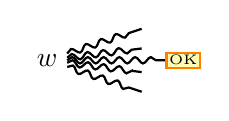
\begin{tikzpicture}[baseline=-0.5ex]
  \node (w) at (0,0) {$w$};
  \draw[thick, decoration={snake, amplitude=.4mm, segment length=2mm, post length=1mm}, decorate] (w) -- (1.2, 0.4);
  \draw[thick, decoration={snake, amplitude=.4mm, segment length=2mm, post length=1mm}, decorate] (w) -- (1.2, 0.15);
  \draw[thick, decoration={snake, amplitude=.4mm, segment length=2mm, post length=1mm}, decorate] (w) -- (1.5, 0) node[right, fill=yellow!30, inner sep=1pt, draw=orange] {\tiny OK};
  \draw[thick, decoration={snake, amplitude=.4mm, segment length=2mm, post length=1mm}, decorate] (w) -- (1.2, -0.15);
  \draw[thick, decoration={snake, amplitude=.4mm, segment length=2mm, post length=1mm}, decorate] (w) -- (1.2, -0.4);
\end{tikzpicture}
\end{center}

\vspace{0.4cm}
\textbf{Esempio:} 
\begin{align*}
    L = \{w \in \{a,b,c\}^* \mid \;& \exists \text{ un'occorrenza di 'c' immediatamente preceduta da } ab \text{ (abc)} \\
    &\text{oppure immediatamente seguita da } ab \text{ (cab)}\}
\end{align*}

\begin{center}
\begin{tikzpicture}[shorten >=1pt, node distance=2.2cm, on grid, auto, thick, scale=0.9, transform shape]
   \node[state, initial, initial text=] (q_0)   {$q_0$};
   \node[state] (q_1) [right=of q_0] {$q_1$};
   \node[state] (q_2) [right=of q_1] {$q_2$};
   \node[state] (q_3) [right=of q_2] {$q_3$};
   \node[state, accepting] (q_4) [right=of q_3] {$q_4$};
   
   \node[state] (q_5) [below=of q_1] {$q_5$};
   \node[state] (q_6) [right=of q_5] {$q_6$};
   \node[state, accepting] (q_7) [right=of q_6] {$q_7$};

   \path[->]
    (q_0) edge node {$*/D$} (q_1)
    (q_1) edge[loop above] node {$a,b,c/D$} (q_1)
    (q_1) edge node {$c/D$} (q_2)
    (q_2) edge node {$a/D$} (q_3)
    (q_3) edge node {$b/b$} (q_4)
    (q_1) edge node[left] {$c/S$} (q_5)
    (q_5) edge node[below] {$b/S$} (q_6)
    (q_6) edge node[below] {$a/a$} (q_7);
    
    % Annotazioni
    \node[orange, above=1cm of q_4, align=center] {Ho trovato \\ (cab)};
    \node[orange, right=2cm of q_7, align=center] {$\longleftarrow$ ho trovato \\ (abc)};
\end{tikzpicture}
\end{center}

\begin{center}
    \begin{tabular}{|c|c|c|c|c|c|c|c|c|c|c|c|c|c|}
    \hline
    * & a & b & a & a & c & b & a & b & c & a & a & b & \dots \\
    \hline
    \multicolumn{7}{c}{} & \multicolumn{3}{c}{$\underbrace{\hspace{1.2cm}}_{\text{(abc)}}$} & \multicolumn{4}{c}{} \\
    \end{tabular}
    \end{center}

\vspace{0.4cm}
\textbf{Grado di non determinismo di $M$:} Data $M$ MDT non deterministica, il suo grado di non determinismo $\delta$ è il massimo numero di scelte possibili per una singola configurazione:
$$ \delta = \max_{\substack{\tilde{q} \in Q \\ \tilde{x} \in \Sigma}} |\{ \tilde{q} \tilde{x} \alpha q \mid \alpha \in \Sigma \cup \{D, S\}, q \in Q \}| $$

Dato $q \in Q, x \in \Sigma$ codifichiamo le transizioni di $M$ (MDT non deterministica) aventi $qx$ come primi 2 elementi utilizzando gli interi da $1$ a $\delta$, possibilmente codificando la stessa transizione con più etichette.
\begin{itemize}
    \item $q_1 \ c \ D \ q_1 \ : \ 1$ \quad \quad $q_1 \ a \ D \ q_1 \ : \ 1, 2, 3$
    \item $q_1 \ c \ D \ q_2 \ : \ 2$
    \item $q_1 \ c \ S \ q_5 \ : \ 3$
\end{itemize}

\textbf{Esempi di possibili computazioni sulla stringa $w = acab$:}
\begin{enumerate}
    \item $1111$, termina in uno stato non finale ($w$ \textit{non accettata})
    \item $11211$, termina in uno stato finale ($w$ \textbf{accettata})
    \item $22322$, termina subito ($w$ \textit{non accettata})
\end{enumerate}

\vspace{0.6cm}
\textbf{Proposizione:} $L$ è accettato da una MDT standard $\iff L$ è accettato da una MDT non deterministica.

\textit{Dimostrazione:}
\begin{itemize}
    \item[$\implies$)] Sia $M$ una MDT standard che accetta $L$. Poiché ogni MDT deterministica è (banalmente) anche una MDT non deterministica, $L$ è accettato da una MDT non deterministica.
    \item[$\impliedby$)] Sia $M$ una MDT non deterministica che accetta $L$ per arresto, con grado di non determinismo di $M = \delta$. Descriviamo una MDT \textit{deterministica} che accetta $L$ per arresto a 3 nastri (per simulare tutte le computazioni parallele di $M$ in modo sistematico):
\end{itemize}

\begin{center}
\begin{tabular}{ll|c|c|c|c|c|l}
\cline{3-7}
3 & & $m_1$ & * & $m_2$ & * & $\dots$ & Generazione delle computazioni di $M$ ($1 \le m_i \le \delta$) \\
\cline{3-7}
\multicolumn{8}{c}{} \\
\cline{3-7}
2 & & * & \multicolumn{4}{c|}{\scriptsize copio l'input ed eseguo $(m_1,\dots,m_K)$} & Simulazione delle computazioni di $M$ \\
\cline{3-7}
\multicolumn{8}{c}{} \\
\cline{3-7}
1 & & \multicolumn{5}{c|}{} & Input \\
\cline{3-7}
\end{tabular}
\end{center}

\vspace{0.8cm}
\subsection{Funzioni Parziali Computabili}

\textbf{Funzione parziale:} Dati $A, B$ insiemi, una funzione parziale da $A$ a $B$ è una funzione da $D$ a $B$, per qualche dominio $D \subseteq A$. \textit{(Cioè potrebbe essere definita solo su una parte di $A$, ad es. $f(x) = \frac{10}{x}$, che non è definita per $x=0$).}

\vspace{0.4cm}
\textbf{Funzione parziale computabile:} Data una funzione parziale $f$ da $A$ a $B$, si dice computabile quando $\exists M$ algoritmo tale che $\forall x \in A$:
\begin{itemize}
    \item Se $x \in \text{Dominio}(f)$, $M$ eseguita su $x$ restituisce in output $f(x)$ $\longrightarrow$ $x \in \text{Dominio}(f)$: $f$ converge su $x$, si scrive \textbf{$f(x)\downarrow$}
    \item Se $x \notin \text{Dominio}(f)$, $M$ su $x$ non termina $\longrightarrow$ $x \notin \text{Dominio}(f)$: $f$ diverge su $x$, si scrive \textbf{$f(x)\uparrow$}
\end{itemize}

Lavoriamo su $\mathbb{N}$ in codifica unaria.

\textbf{Definizione:} $f$ funzione parziale da $\mathbb{N}^k \to \mathbb{N}$ si dice \textbf{parziale $\tau$-ricorsiva} quando $\exists M$ MDT che, $\forall \vec{x} \in \mathbb{N}^k$:
\begin{itemize}
    \item Se $f(\vec{x})\downarrow$ allora l'esecuzione di $M$ su $\vec{x}$ termina con $f(\vec{x})+1$ "uni" sul nastro.
    \item Se $f(\vec{x})\uparrow$ allora l'esecuzione di $M$ su $\vec{x}$ non termina su $\vec{x}$.
\end{itemize}

\vspace{0.4cm}
\textbf{Tesi di Church per funzioni parziali $\tau$-ricorsive:} La classe delle funzioni parziali computabili coincide con la classe delle funzioni parziali $\tau$-ricorsive.

\vspace{0.4cm}
\textbf{Proposizione:} $\forall M$ MDT deterministica, $\forall K \in \mathbb{N} \ \exists!$ funzione parziale computabile $f: \mathbb{N}^k \to \mathbb{N}$ tale che $M$ calcola $f$.

\textit{Dimostrazione:}
Definisco $f$ funzione parziale da $\mathbb{N}^k$ in $\mathbb{N}$ come segue: \\
$\forall \vec{x} \in \mathbb{N}^k$, eseguo $M$ su $\vec{x}$:
\begin{itemize}
    \item Se $M$ termina, $f(\vec{x})$ è data in unario dal numero di "uni" che si trovano sul nastro al termine dell'esecuzione.
    \item Se $M$ non termina, $f(\vec{x})\uparrow$. Questo ci dice che ad ogni $M$ corrisponde (in modo univoco) una funzione $f$ ($M \longleftrightarrow f$).
\end{itemize}